\chapter{Machine Learning}

\section{\textit{Gio 3 novembre - Lezione 12}}
\section{Introduction to Machine Learning}

\subsection{Topics}

\begin{enumerate}
	\item Introduction to machine learning
		\begin{enumerate}
			\item Basic concepts: loss, overfit, underfit
			\item Examples of linear regression, boosted decision trees
			\item Exercise with colab, numpy, scikit
		\end{enumerate}
	\item Deep Neural Networks
			\begin{enumerate}
			\item Basic FeedForward networks and backpropagation
			\item Importance of depth, gradient descent, optimizers
			\item Introduction to tools and first exercises
			\end{enumerate}
	\item Convolutional and Recurrent networks
		\begin{enumerate}
			\item Reduction of complexity with invariance: RNN and CNN
			\item CNN exercise
		\end{enumerate}
	\item Autoencoders and Generative Adversarial Networks
		\begin{enumerate}
			\item GAN exercises
		\end{enumerate}
	\item Graph Neural Networks
		\begin{enumerate}
			\item PointCloud exercise
		\end{enumerate}
\end{enumerate}

\subsection{Machine Learning Basics}
\textbf{Wikipedia:} Machine learning (ML) is a field of inquiry devoted to understanding and building methods that \textit{'learn'}, that is, methods that leverage data to improve performance on some set of tasks. It is seen as a part of \textit{artificial intelligence}. Machine learning algorithms build a model based on sample data, known as training data, in order to make predictions or decisions \textbf{without being explicitly programmed to do so}. Machine learning algorithms are used in a wide variety of applications, such as in medicine, email filtering, speech recognition, and computer vision, where it is difficult or unfeasible to develop conventional algorithms to perform the needed tasks.\\

Noi siamo abituati a dare al computer degli ordini imperativi.\\

In experimental and applied physics examples are everywhere...
\begin{itemize}
	\item Particle identification and kinematic measurement
	\item Signal to background discrimination (BDT and DNN are very popular in HEP experiments)
	\item Computer assisted processing of medical exams (ECG, CT, etc...)
	\item Processing of astrophysics data
\end{itemize}

\subsection{Types of typical ML problems}


\begin{itemize}
	\item \textbf{Classification:} which category a given input belongs to. 
	\item \textbf{Regression:} value of a real variable given the input.
	\item \textbf{Clustering:} group similar samples
	\item \textbf{Anomaly detection:} identify inputs that are “different” from the others
	\item \textbf{Generation/synthesis of samples:} produce new samples, similar to the original data, starting from noise/random numbers
	\item \textbf{Denoising:} remove noise from an input dataset
	\item \textbf{Transcriptions:} describe in some language the input data
	\item \textbf{Translations:} translate between languages
	\item \textbf{Encoding and decoding:} transform input data to a different representation
	\item ...many more...
\end{itemize}

\subsection{Function approximation}

The goal of a ML algorithm is to approximate an unknown function (often related to some Probability Density Function of the data) given some example data.\\
The function is often $ f(\textbf{x}): R^n \rightarrow R^m$ (in many simple problems $m=1$)
\begin{itemize}
	\item In\textbf{classification} we try to approximate the probability for each example, given the inputs represented as a vector \textbf{x}, to belong to a given category (y) (e.g. the probability to be a LHC Higgs signal event vs a Standard Model background one)
	\item In \textbf{regression} we approximate the function that given the inputs (x) returns the value of the variable to predict (y) (e.g. given the data read from some particle detectors, estimate the particle energy).
\end{itemize}

\begin{figure}[ht]
	\centering
	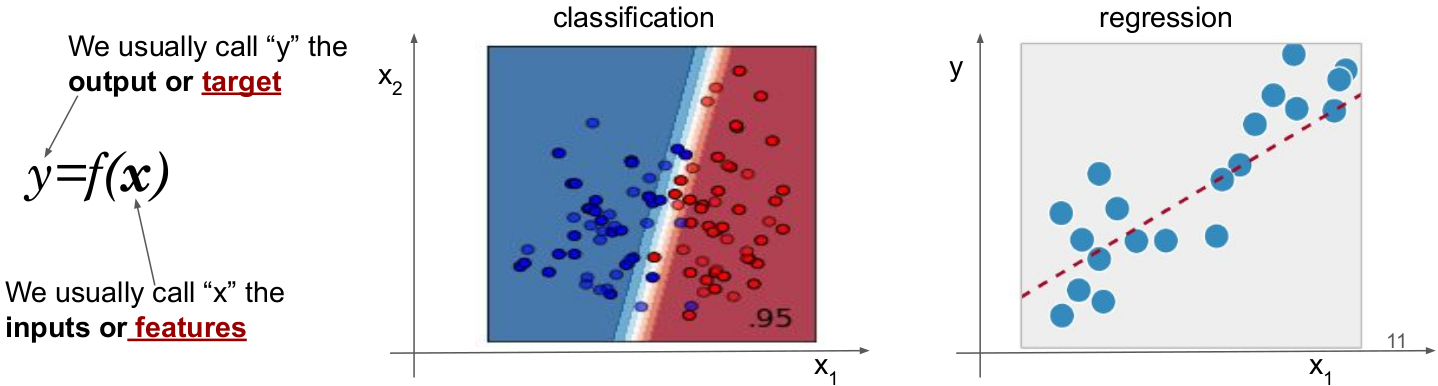
\includegraphics[width=1\textwidth]{figure_ml/function_approx.png}
\end{figure}
\FloatBarrier

\subsection{Model and Hyper-parameters}
A model for the functions that can be used to approximate the “f(x)” must be defined. The model can be something simple (e.g. sum of polynomials up to degree N) or more complex (e.g. all the functions that could be coded in M lines of C++).\\
Different ML techniques are based on different “models”:
\begin{itemize}
	\item Each technique (“class of model”) further allow to specify the exact model
	\item The parameters describing the exact model are called “hyper-parameters” (e.g. the degree N of the polynomial, or the maximum number of C++ line M can be considered hyper
	parameters)
\end{itemize}

We will see example of techniques with different models and complexity: (Linear regression, Decision trees, Principal Component Analysis, Nearest Neighbor, Artificial Neural Networks).

\subsection{Parameters}

A specific model typically have parameters (e.g. the coefficients of the polynomials or the characters of the 10 lines of C++).
Parameters are what we learn from data in the “training phase”.
Different models or similar model with different hyper-parameters settings have different n.d.o.f. in the parameters phase space.
\begin{equation*}
	y(x) = ax + bx^2 + cx^3 + d \qquad \qquad	\text{(a, b, c, d are the parameters)}
\end{equation*}

I parametri sono la cosa che voglio imparare nella fase di training. Mentre gli iperparametri li fisso prima di allenare il modello facendogli vedere i dati, i parametri sono invece proprio quelli che imparo.

\section{Objective function}
DObbiamo stabilire una metrica per dire quanto è buona la nostra approssimazione, dati gli esempi su ci ci stamo allenando.\\

A goal for what is “a good approximation” have to be defined This is called objective function (or loss function or error function …) Is a function that returns higher(or lower) value depending how good or bad the approximation is. Loss functions have to be minimized.\\
Examples of loss functions:
\begin{itemize}
	\item Classification problems: binary cross entropy
	\item Regression problems: Mean Square Error (i.e. the chi2 with sigma=1, I hope you are not surprised by this choice!)
\end{itemize}

The process is not very different from a typical phys-lab1 chi2 fit… but the number
of parameters can be several orders of magnitude larger ($10^3$ to $10^6$).

\subsubsection{Objective function: binary cross entropy}
In classification problems the function to approximate is typically $R^n \rightarrow [0,1]$, Where, for example, 0 means background and 1 means signal.\\
The binary cross entropy is defined as follows ($\hat{y}_i$ is the output of the classifier)
 
\begin{figure}[h]
	\centering
	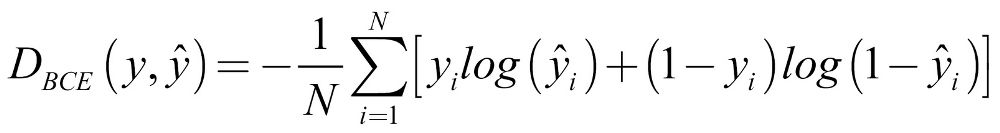
\includegraphics[width=0.5\textwidth]{figure_ml/D_bce.png}
\end{figure}
\FloatBarrier
The above function has large value when an example with y=1 is classified as 
a  $\hat{y}_i \sim 0$ and no loss when $\hat{y}_i \sim 1$. Viceversa if y=0 …\\
Minimizing the binary cross-entropy we maximize the likelihood in a process with 0/1 outcome (where the output of the function is interpreted as a probability).
 
\begin{figure}[h]
	\centering
	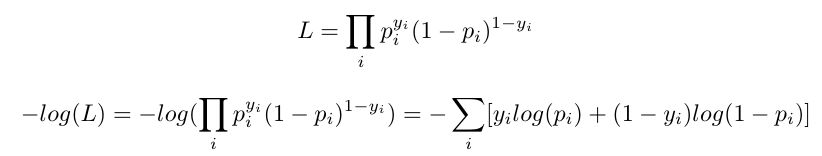
\includegraphics[width=0.65\textwidth]{figure_ml/L_bce.png}
\end{figure}
\FloatBarrier

\subsection{Learning / Training}
For a given model, and given set of hyper-parameters, how do we infer the parameters that minimize the objective function? The idea of ML is to get the parameters from “data” in a so called “training” step. Each ML technique has a different approach to training.\\
Different types of training:
\begin{itemize}
	\item \textbf{Supervised}: i.e. for each example we know the correct answer
	\item \textbf{Unsupervised}: we do not know “what is what”, we ask the ML algorithm to learn the probability density function of the examples in the features (i.e. the inputs!) space
	\item \textbf{Reinforcement learning}: have agents playing a punishment/reward game
\end{itemize}

\subsubsection{Supervised learning}

We want to teach something we (the supervisors) already know (at least on the training samples). For each example we need to have the “right answer” / “truth”, for example:

\begin{itemize}
	\item Labels telling if a given example signal or background, typically $y \in{0,1}$ (e.g. 0=background, 1=signal)
	\item Labels classifying the content of an image (multiple labels are possible)
	\item One-hot encoding used when multiple categories are possible:
		\begin{itemize}
			\item y=[0 1 0 0] means an element of the “2nd class”, y=[0 0 0 1] means an element of the “4th class”
			\item Much better than $y\in {0,1,2,3}$ if class “2” has no reason to be closer to “3” than to “0”
			\item Allows interpretation of the output (e.g. [0.1 0.3 0.06 0.001 ] as the probability to belong to each of the classes
			\item Allow for multi labeling (i.e. one sample can be belong to more than one category)
		\end{itemize}
	\item In regression problems the “truth” is the “correct values” of some quantity
		\begin{itemize}
			\item e.g. generated energy of a particle in a detector simulation
		\end{itemize}
\end{itemize}

Sample can be labelled in various ways:
\begin{itemize}
	\item Humans labelling existing data
	\item Data being “generated” from known functions (e.g. simulations)
\end{itemize}

Learn the probability of the label y, given the input \textbf{x}, i.e. P(y|\textbf{x})

\begin{figure}[ht]
	\centering
	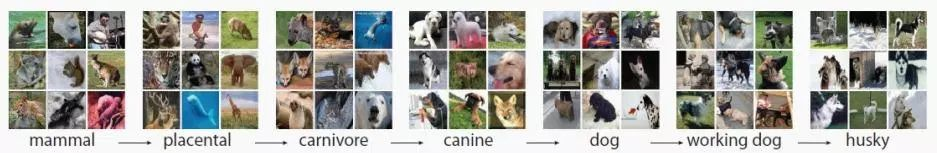
\includegraphics[width=1\textwidth]{figure_ml/supervised_learning.png}
\end{figure}
\FloatBarrier

\begin{figure}[ht]
	\centering
	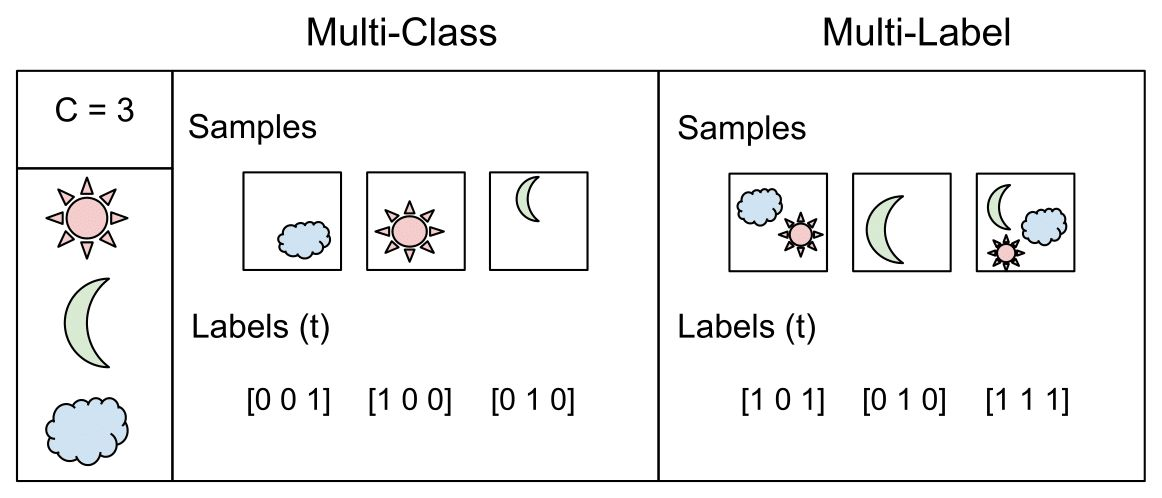
\includegraphics[width=0.4\textwidth]{figure_ml/multi_class.png}
\end{figure}
\FloatBarrier

\subsubsection{Unsupervised learning}

\begin{wrapfigure}{r}{0.5\textwidth}
	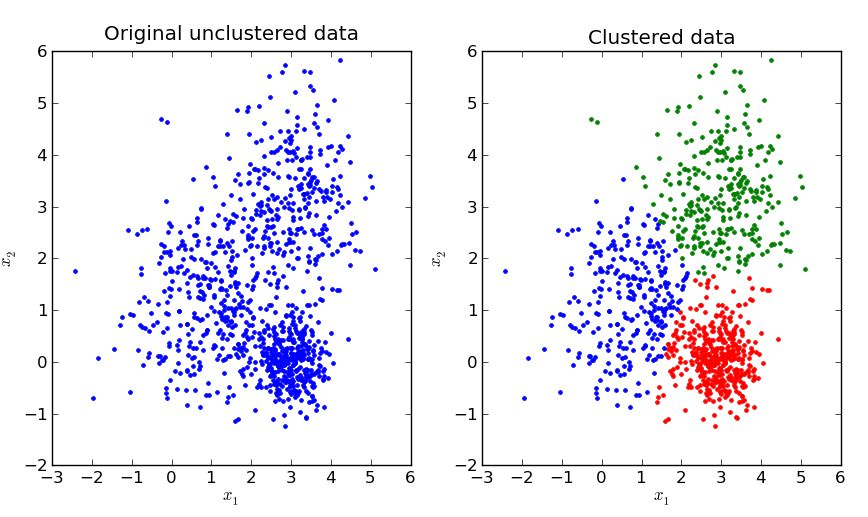
\includegraphics[width=0.5\textwidth]{figure_ml/unsupervised.png}
\end{wrapfigure} 

Often we do not have labels (or we have labels only for few data points). Unsupervised learning techniques allow to train networks that can perform
similar tasks as the supervised ones, e.g.

\begin{itemize}
	\item Classification of “common” patterns (clustering)
	\item Dimensionality reduction, compression
	\item Prediction of missing inputs
	\item Anomaly detection
\end{itemize}



In practice learn the Probability Density Function of the data, independently of any “label” variable, i.e. P(\textbf{x})

\subsubsection{Supervised vs unsupervised}

Supervised and unsupervised are not as different as one would imagine, in fact.\\
Unsupervised P(\textbf{x}) can be seen as n supervised problems, one for each feature of the input vector

\begin{figure}[ht]
	\centering
	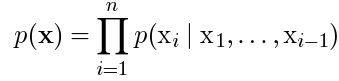
\includegraphics[width=0.4\textwidth]{figure_ml/s_vs_u.png}
\end{figure}
\FloatBarrier

Supervised P(y | \textbf{x}) can also be computed, if we treat y as an “\textbf{x}” in unsupervised learning deriving hence $p(\textbf{x},y)$
, as


\begin{figure}[ht]
	\centering
	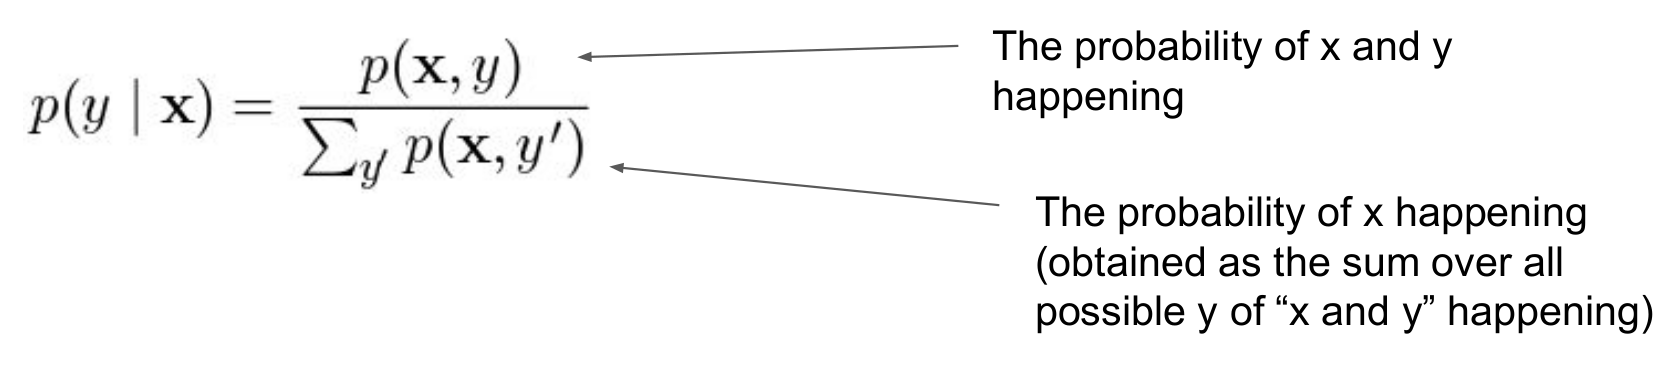
\includegraphics[width=0.8\textwidth]{figure_ml/s_vs_u2.png}
\end{figure}
\FloatBarrier

\subsubsection{Reinforcement learning (not covered in this lectures)}
\begin{wrapfigure}{r}{0.5\textwidth}
	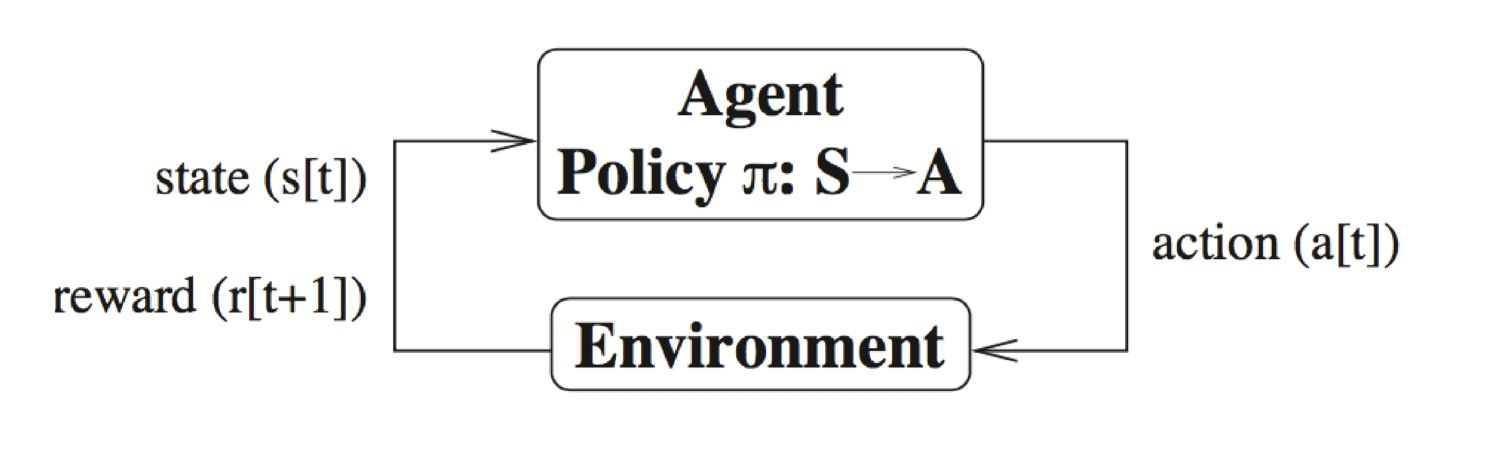
\includegraphics[width=0.5\textwidth]{figure_ml/reinforcement_learning.png}
\end{wrapfigure} 

Applies to “agents” acting in an “environment” that updates their state.\\
It is similar to supervised learning as a “reward” has to be calculated. The supervisor anyhow doesn’t necessarily know what is the best action to perform in a given state to interact with the environment, it just computes the final reward.\\
Learn to make best decision in a given situation
\begin{itemize}
	\item The right move in chess or go match
	\item Drive a car in the traffic
	\item Etc.
\end{itemize}


\subsection{Capacity and representational power}

\begin{wrapfigure}{r}{0.3\textwidth}
	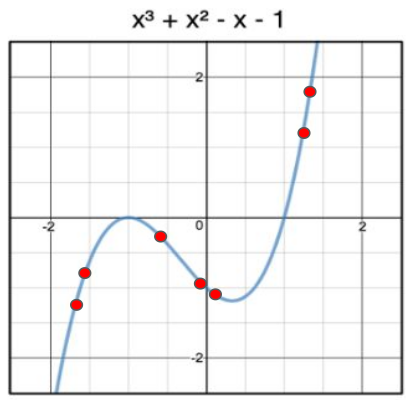
\includegraphics[width=0.3\textwidth]{figure_ml/capacity.png}
\end{wrapfigure} 

Different models (i.e. ML techniques/hyper-parametersvalues) allow to represent different type of functions.
Models with more free parameters typically can approximate a larger number
of functions (or can better approximate a given function) => higher capacity.
Remember: we do not know the actual function to approximate, we just want
to learn from examples.
With limited samples we have a tradeoff to
handle: accuracy in representation vs generalization of the results.\\


\noindent
\textbf{Underfitting:} the sample is badly represented.\\
\textbf{Overfitting} / Appropriate capacity are less obvious to define. (Lack of “generalization” $\rightarrow$ overfitting).

\begin{figure}[ht]
	\centering
	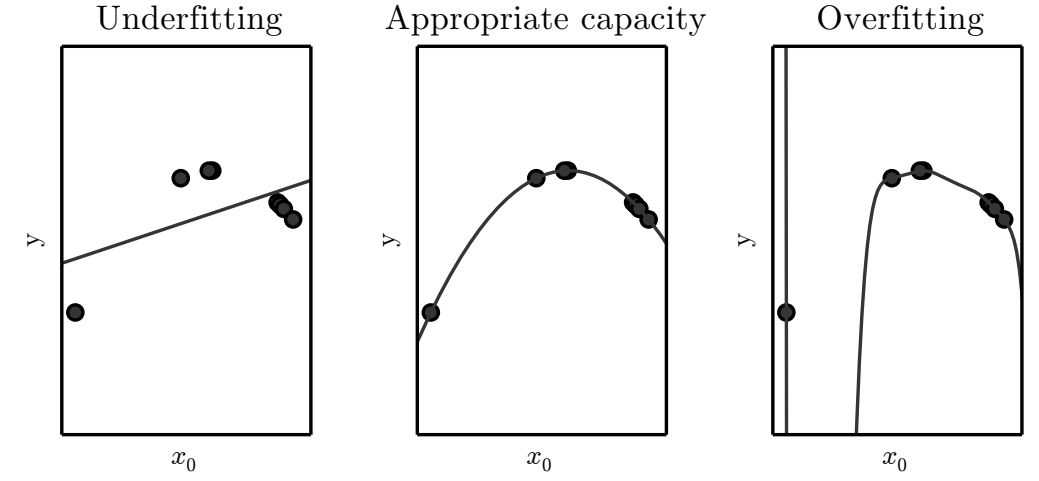
\includegraphics[width=0.6\textwidth]{figure_ml/u_a_o.png}
\end{figure}
\FloatBarrier

Typical method is to check on independent sample for the same process (Or just split your sample in two and use only half for training).

\begin{figure}[ht]
	\centering
	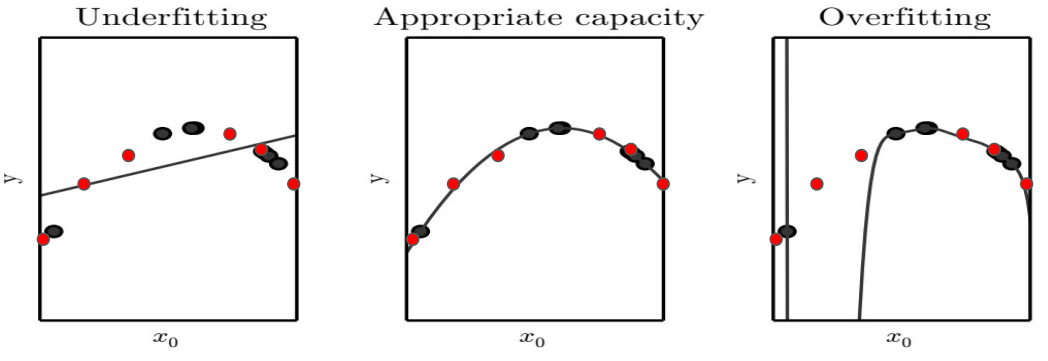
\includegraphics[width=0.6\textwidth]{figure_ml/u_a_o2.png}
\end{figure}
\FloatBarrier

\subsection{Generalization}

We can compare the accuracy between the “training” sample and the “generalization/validation” sample.\\

\begin{figure}[ht]
	\centering
	\begin{subfigure}{.5\textwidth}
		\centering
		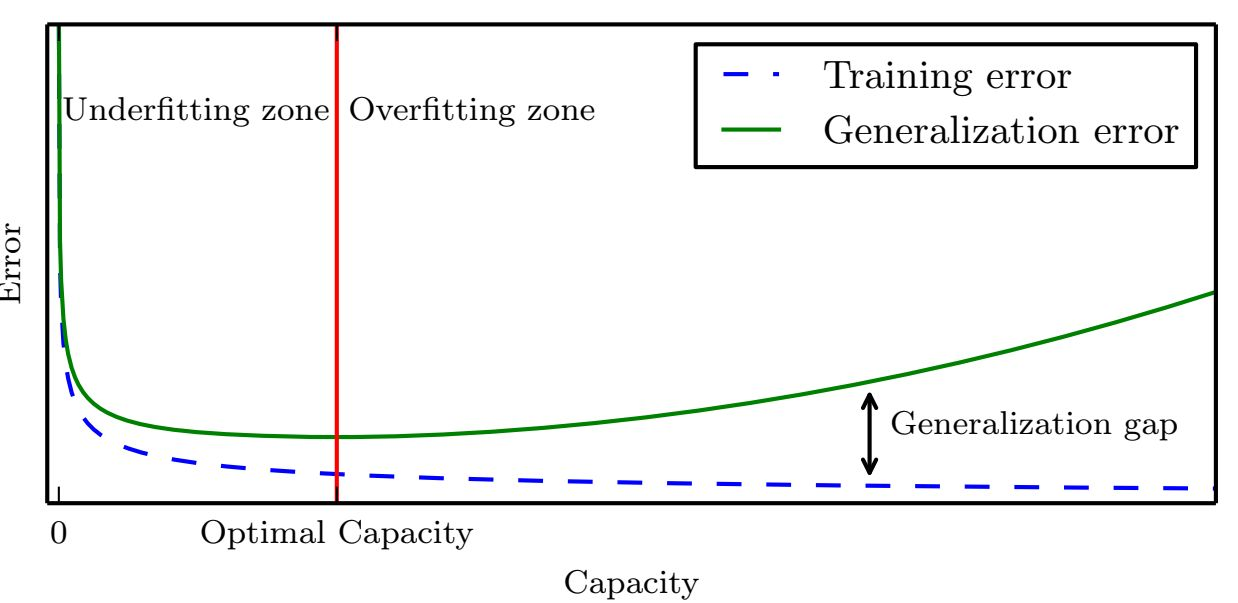
\includegraphics[width=1\linewidth]{figure_ml/generalization.png}
	\end{subfigure}%
	\begin{subfigure}{.5\textwidth}
		\centering
		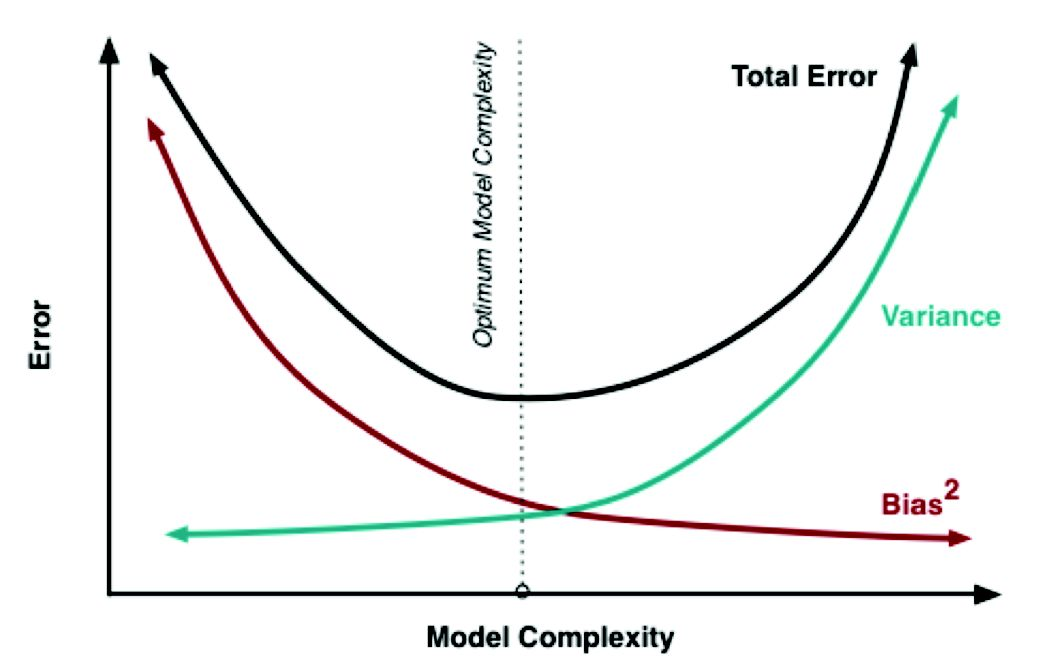
\includegraphics[width=1\linewidth]{figure_ml/generalization2.png}
	\end{subfigure}

\end{figure}



Bias/variance trade-off
\begin{itemize}
	\item y: function (with random noise)
	\item h(x): approximated function
\end{itemize}


\begin{figure}[ht]
	\centering
	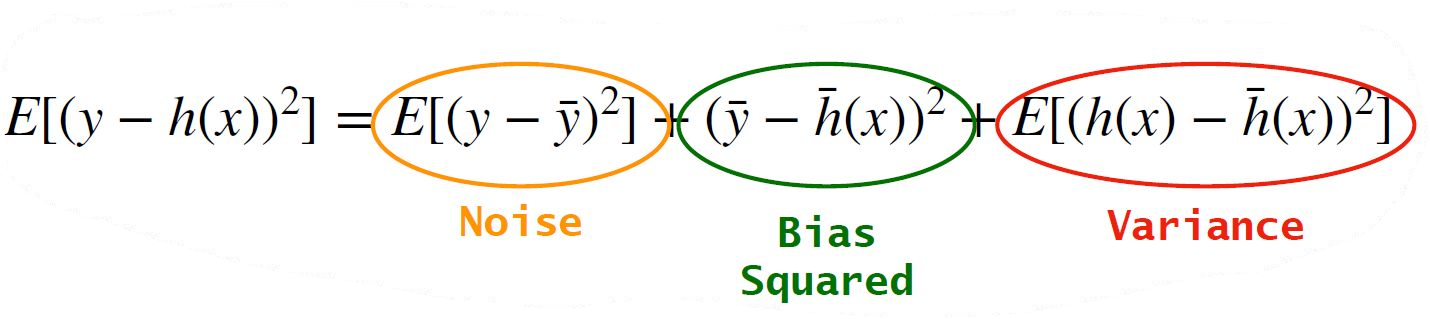
\includegraphics[width=0.45\textwidth]{figure_ml/generalization3.png}
\end{figure}
\FloatBarrier


\subsection{Regularization}

\begin{wrapfigure}{r}{0.45\textwidth}
	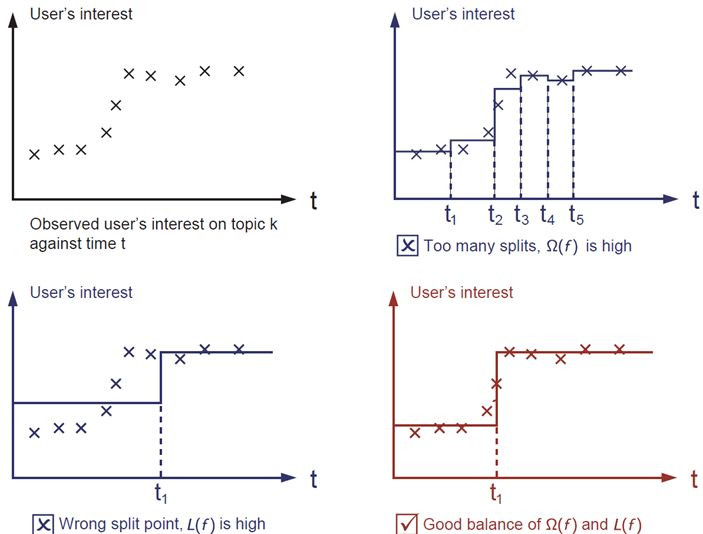
\includegraphics[width=0.45\textwidth]{figure_ml/regularization.png}
\end{wrapfigure} 

Vogliamo evitare che "impari a memoria" il set.\\
In order to control the “generalization gap”. the objective function can be modified adding a regularization term (Introduce a “cost” in increasing the capacity of the model or in accessing some parts of the model-parameters space).\\

the examples in training dataset can be increased with augmentation techniques:

\begin{itemize}
	\item Adding stochastic noise to existing examples
	\item Transforming the existing examples with transformation that are known to be invariant 	for the solution we look for
\end{itemize}


\url{https://xgboost.readthedocs.io/en/latest/tutorials/model.html}



\subsection{Hyperparameters(model) optimization}

It is normal to have to test a few, if not several, configurations in the model hyper-parameter space:
\begin{itemize}
	\item Scans of hyper-parameters are often performed
	\item Different techniques used
\end{itemize}


Effectively a “second” minimization is done

\begin{itemize}
	\item First minimization is on the parameter => minimize on the “training dataset”
	\item Second minimization is on the hyper-parameters => minimize on the “validation dataset”
\end{itemize}

A third dataset (“test dataset”) is then also needed

\begin{itemize}
	\item To assess the performance of the algorithm in an unbiased way
	\item To make an unbiased prediction of the algorithm output
\end{itemize}


Original dataset is typically split in uneven parts to be used as \textit{training}, \textit{validation} and \textit{test}

\begin{figure}[ht]
	\centering
	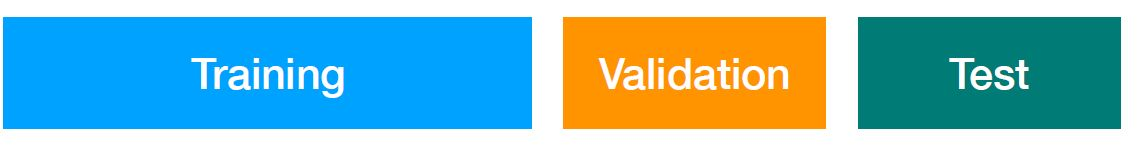
\includegraphics[width=0.7\textwidth]{figure_ml/hyperparams_optimization.png}
\end{figure}
\FloatBarrier

\subsection{K-folding cross validation}

If the sample is statistically limited, splitting in 3 chunks means loosing
examples.\\
With K-folding, “K” independent trainings are performed, each using a
different chunk of data for “training” and for “testing” (and another one for
validation if a hyper parameter scan is performed)

\begin{figure}[ht]
	\centering
	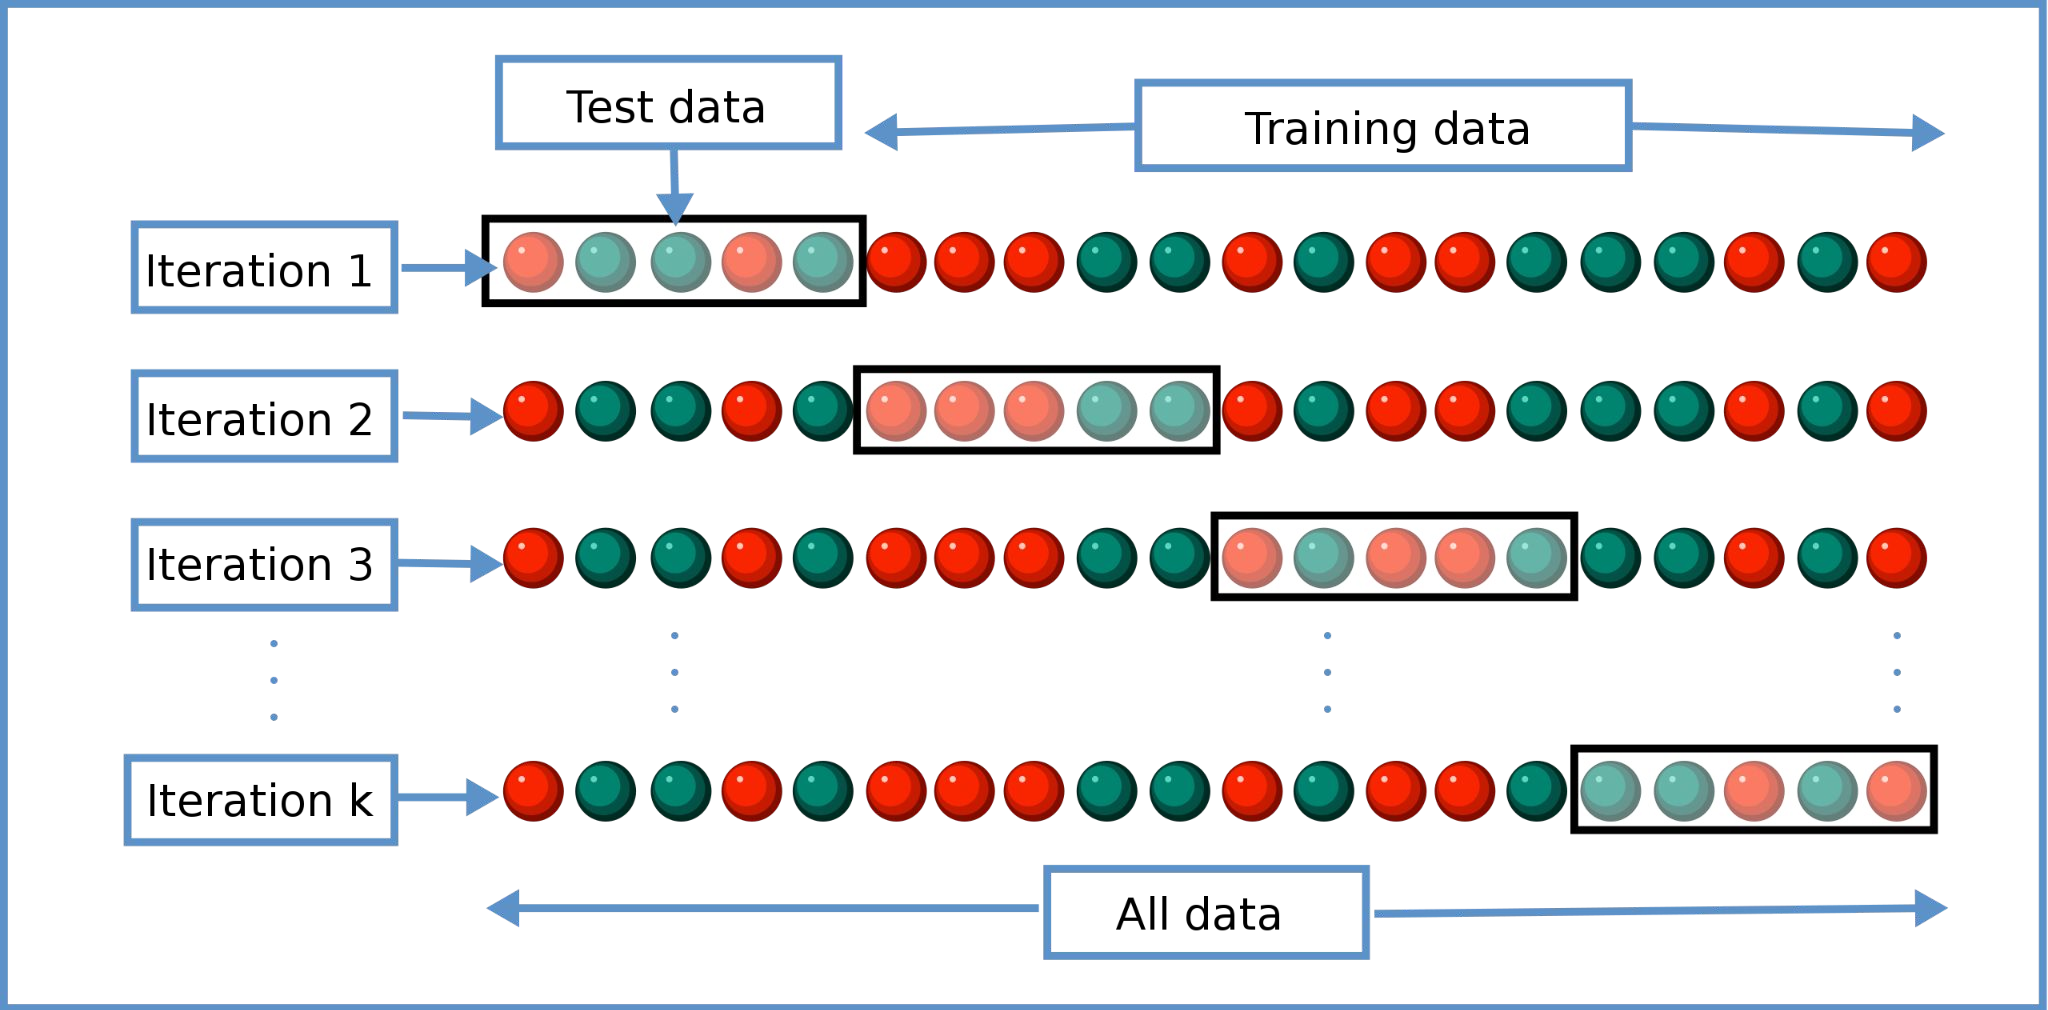
\includegraphics[width=0.7\textwidth]{figure_ml/k-folding.png}
	\caption{Nella figura i dati sono divisi solo in 2 (test e training), ma si possono dividere in 3 come abbiamo visto prima}
\end{figure}
\FloatBarrier

\subsection{Inference}

A ML model that has been trained can than be used to act on some new data (or on the test dataset if a prediction has to be made).
The evaluation of the algorithm output on the “unseen” data is called inference. From a computing time point of view inference is usually much faster than training.

\subsection{Accuracy, Precision, Sensitivity, Specificity}

\begin{figure}[ht]
	\centering
	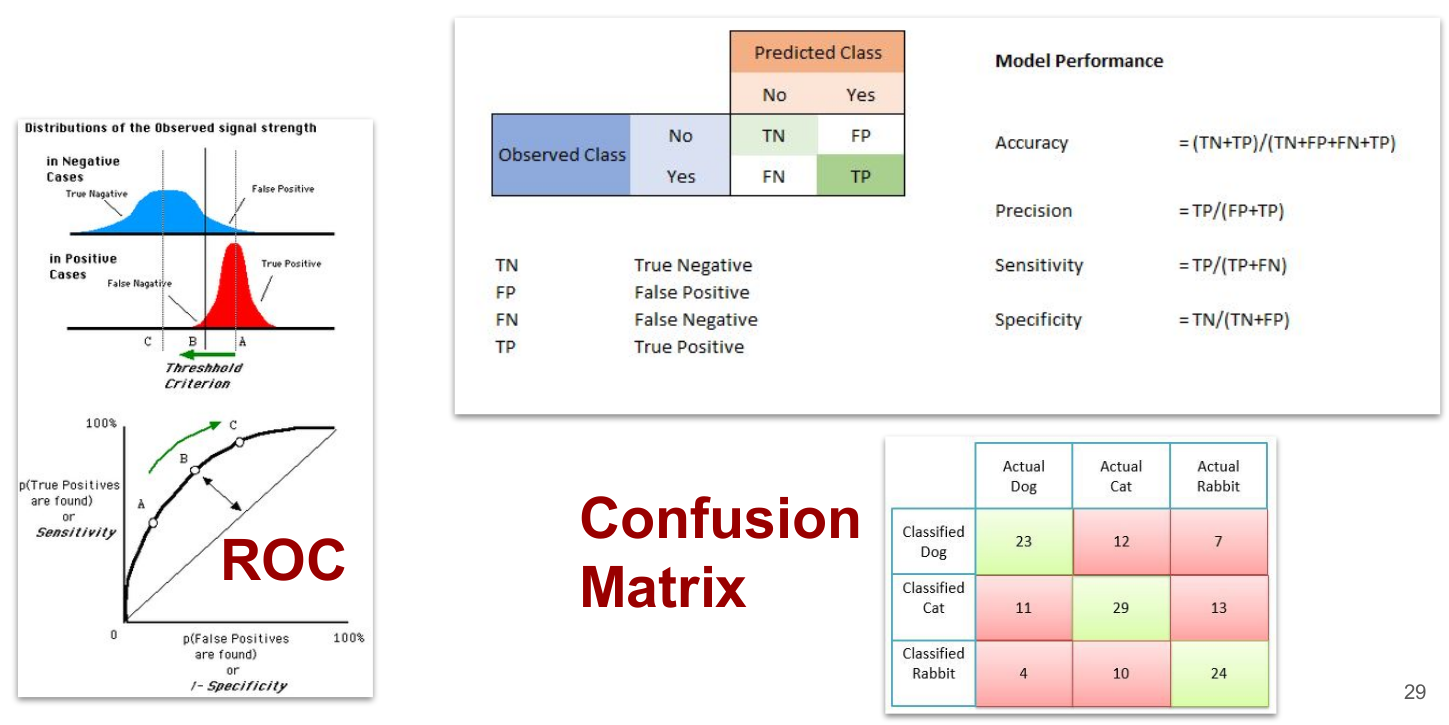
\includegraphics[width=1\textwidth]{figure_ml/apss.png}
\end{figure}
\FloatBarrier


\section{Examples of ML techniques}

\subsection{Linear regression (Supervised)}

Solve a regression problem, i.e. predict the value of y when \textbf{x} is given. Approximate an unknown “y=f(\textbf{x})” given some examples of (y,\textbf{x})\\

\textbf{Model:} $y=w_ix_i$ , i.e. the function is a linear combination of the input parameters\\

\textbf{Parameters:} $ w_i$\\

Let’s suppose we have m examples in the form of pairs $(\textbf{x},y)_j$\\

The \textbf{objective function} can be the mean squared error, MSE=$|y_j - w_i x_{ij} |^2/m$\\

\textbf{Training}: find the parameters $w_i$ that minimize the MSE on the given dataset. Linear regression have an analytical solution (i.e. a minimum for the MSE) that can be computed by requiring the gradient of the MSE to be zero (if you want to see the math \url{https://en.wikipedia.org/wiki/Linear_regression#Least-squares_estimation_and_related_techni
ques}.

We could increase the \textbf{capacity} of the model using polynomials instead of linear functions.The number of parameters would increase as we now would have the second order
coefficients too
\subsection{Principal Component Analysis (aka PCA) (Unsupervised)}

\begin{wrapfigure}{r}{0.45\textwidth}
	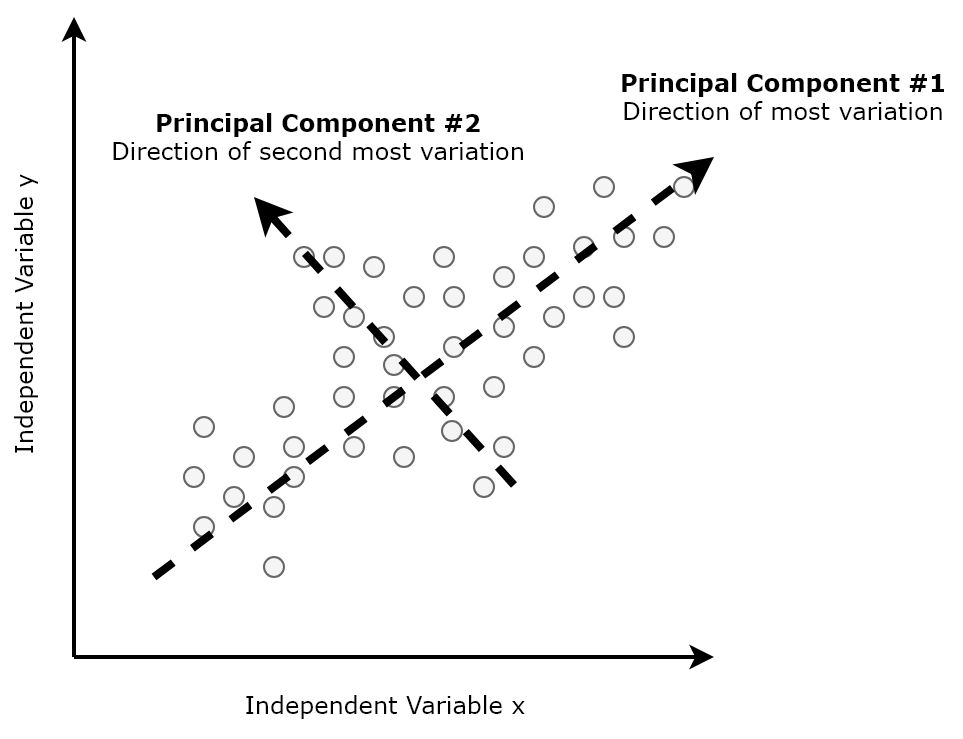
\includegraphics[width=0.45\textwidth]{figure_ml/pca.png}
\end{wrapfigure} 

Orthogonal transformation of the input phase space such that
\begin{itemize}
	\item The first transformed coordinate has maximum variance 
	\item The 2nd transformed coordinated has 2nd max variance
	\item etc.
\end{itemize}

Can be computed as the eigenvalue decomposition of the
covariance matrix

\begin{figure}[ht]
	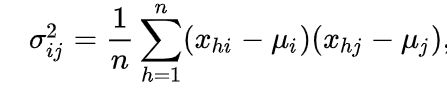
\includegraphics[width=0.35\textwidth]{figure_ml/pca_covariance.png}
\end{figure}
\FloatBarrier

Useful to transform the data in a normalized form (scaling by the variance of each component).\\
Reduce dimensionality (by taking only first N components) capturing only the largest deviations from the mean value.\\

More complex dimensionality reduction Manifold Learning:\url{https://github.com/jakevdp/PythonDataScienceHandbook/blob/master/notebooks/05.10-Manifold-Learning.ipynb}

\subsubsection{Nearest neighbors}

A very powerful way to do classification or regression is to look at points in the training datasets that are close to sample
to evaluate.
Multiple neighbors can be used for
a more stable evaluation.
On large dataset it could be a problem to keep all training points for the evaluation phase.


\begin{figure}[ht]
	\centering
	\begin{subfigure}{.5\textwidth}
		\centering
		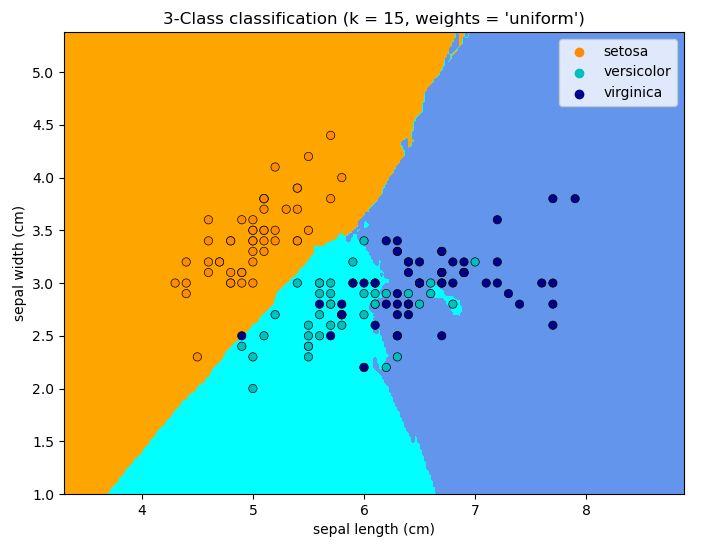
\includegraphics[width=1\linewidth]{figure_ml/nn.png}
	\end{subfigure}%
	\begin{subfigure}{.5\textwidth}
		\centering
		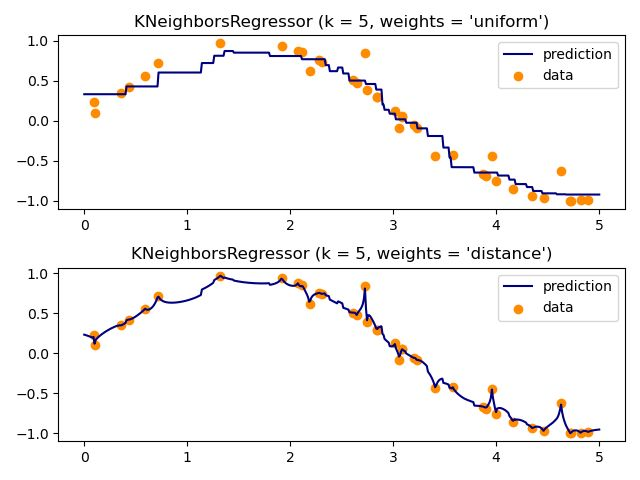
\includegraphics[width=1\linewidth]{figure_ml/nn2.png}
	\end{subfigure}
	\caption{
		Figures from \url{https://scikit-learn.org/stable/modules/neighbors.html}.
	}
\end{figure}


\subsection{Decision trees}

The functions used in the “model” are decision trees, each node has a pass/fail condition on some input variable.\\
Classification and regression trees (CART)
\begin{itemize}
	\item Examples are categorized based on individual “cuts” on a single input feature
	\item A score is given in each leaf
\end{itemize}
Trees can have different depths (depth is an hyper-parameter)

\begin{figure}[ht]
	\centering
	\begin{subfigure}{.5\textwidth}
		\centering
		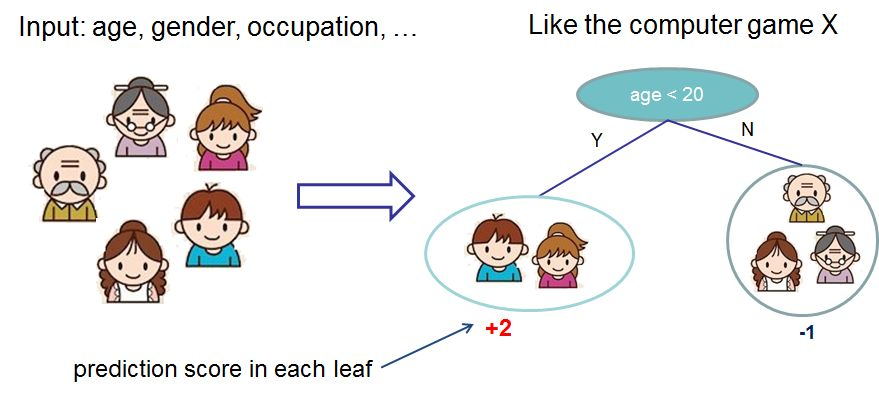
\includegraphics[width=1\linewidth]{figure_ml/decision_trees.png}
	\end{subfigure}%
	\begin{subfigure}{.5\textwidth}
		\centering
		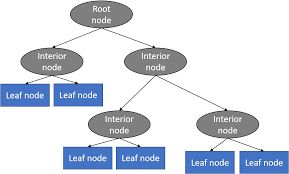
\includegraphics[width=1\linewidth]{figure_ml/decision_trees2.png}
	\end{subfigure}
\end{figure}



\url{https://xgboost.readthedocs.io/en/latest/tutorials/model.html}


\subsection{Ensembles of trees}

A single tree is typically not a very performant.\\
Combine multiple trees (\#trees is an hyperpar)
\begin{itemize}
	\item Random forest (bagging)
	\item Gradient boosting
	\item Adaptive boosting
\end{itemize}

\begin{figure}[ht]
	\centering
	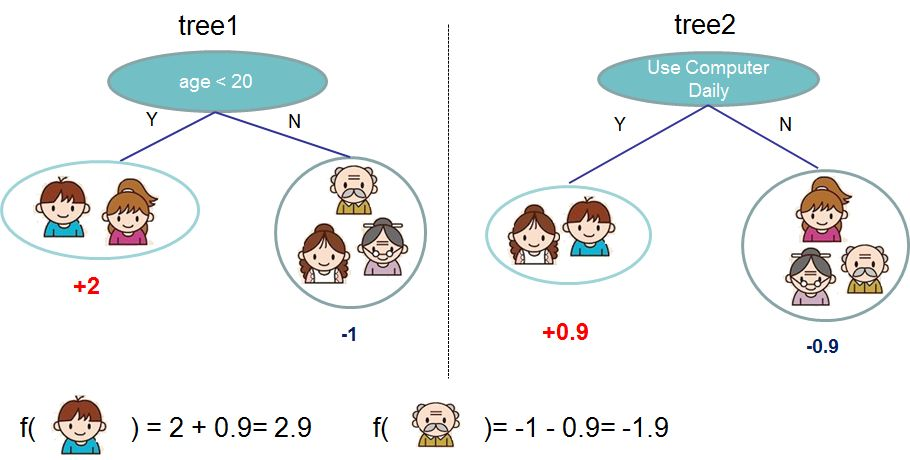
\includegraphics[width=0.5\textwidth]{figure_ml/trees.png}
\end{figure}
\FloatBarrier

\begin{figure}[ht]
	\centering
	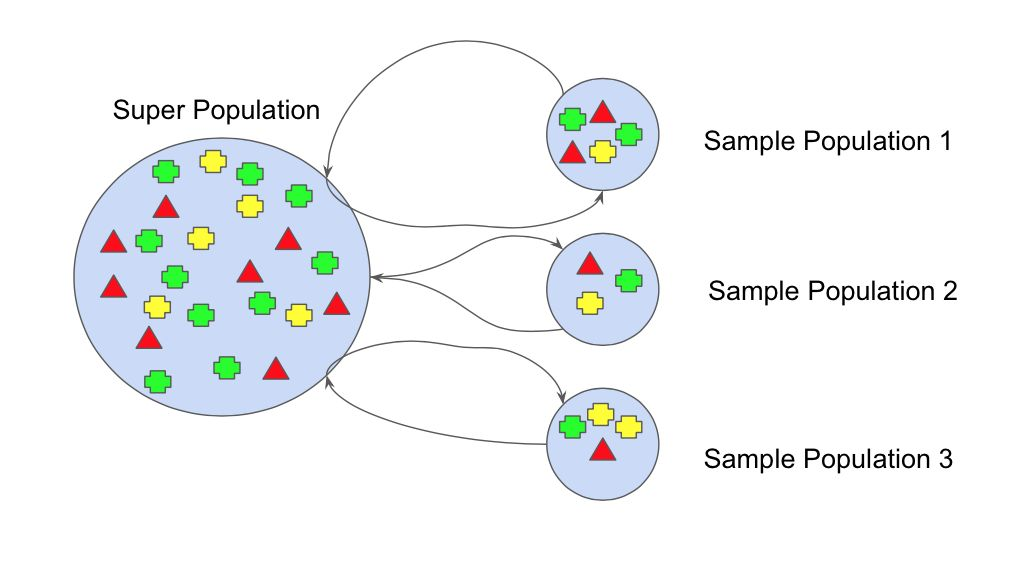
\includegraphics[width=0.5\textwidth]{figure_ml/bagging.png}
	\caption{Bagging}
\end{figure}
\FloatBarrier



\begin{figure}[ht]
	\centering
	\begin{subfigure}{.5\textwidth}
		\centering
		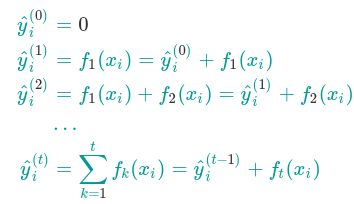
\includegraphics[width=1\linewidth]{figure_ml/g_b.png}
	\end{subfigure}%
	\begin{subfigure}{.5\textwidth}
		\centering
		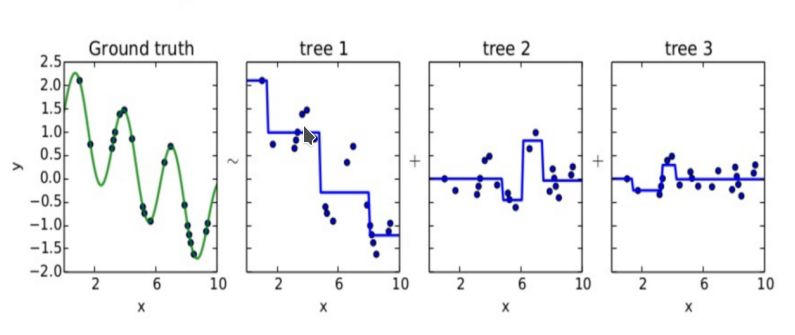
\includegraphics[width=1\linewidth]{figure_ml/g_b2.png}
	\end{subfigure}
	\caption{Gradient Boosting}
\end{figure}



\subsection{Limitations of decision trees}
Cuts are axis aligned!\\
Classification of \textbf{x1 > x2} is a hard problem for a decision tree


\begin{figure}[ht]
	\centering
	\begin{subfigure}{.4\textwidth}
		\centering
		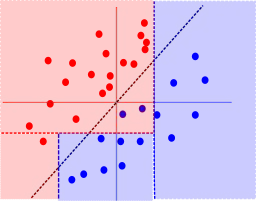
\includegraphics[width=0.9\linewidth]{figure_ml/limitations_trees.png}
	\end{subfigure}%
	\begin{subfigure}{.6\textwidth}
		\centering
		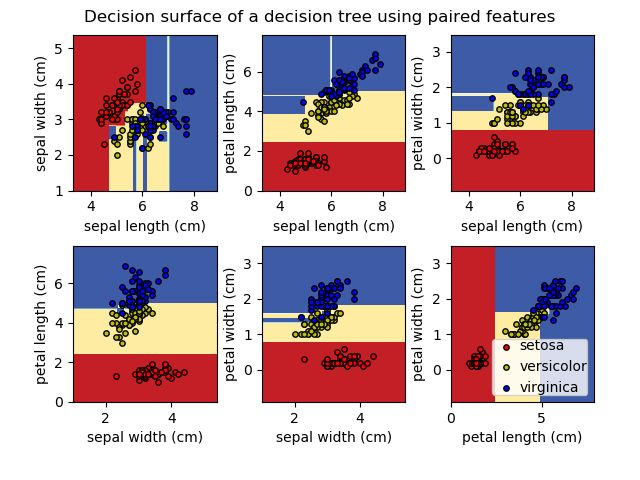
\includegraphics[width=0.9\linewidth]{figure_ml/limitations_trees2.png}
	\end{subfigure}
\end{figure}




\subsection{Many more ML techniques!}

Scikit-learn library offers many ML techniques implementation in python.\\
\url{https://scikit-learn.org/stable/auto_examples/classification/plot_classifier_comparison.html#sphx-glr-auto-examples-classification-plot-classifier-comparison-py}

\begin{figure}[ht]
	\centering
	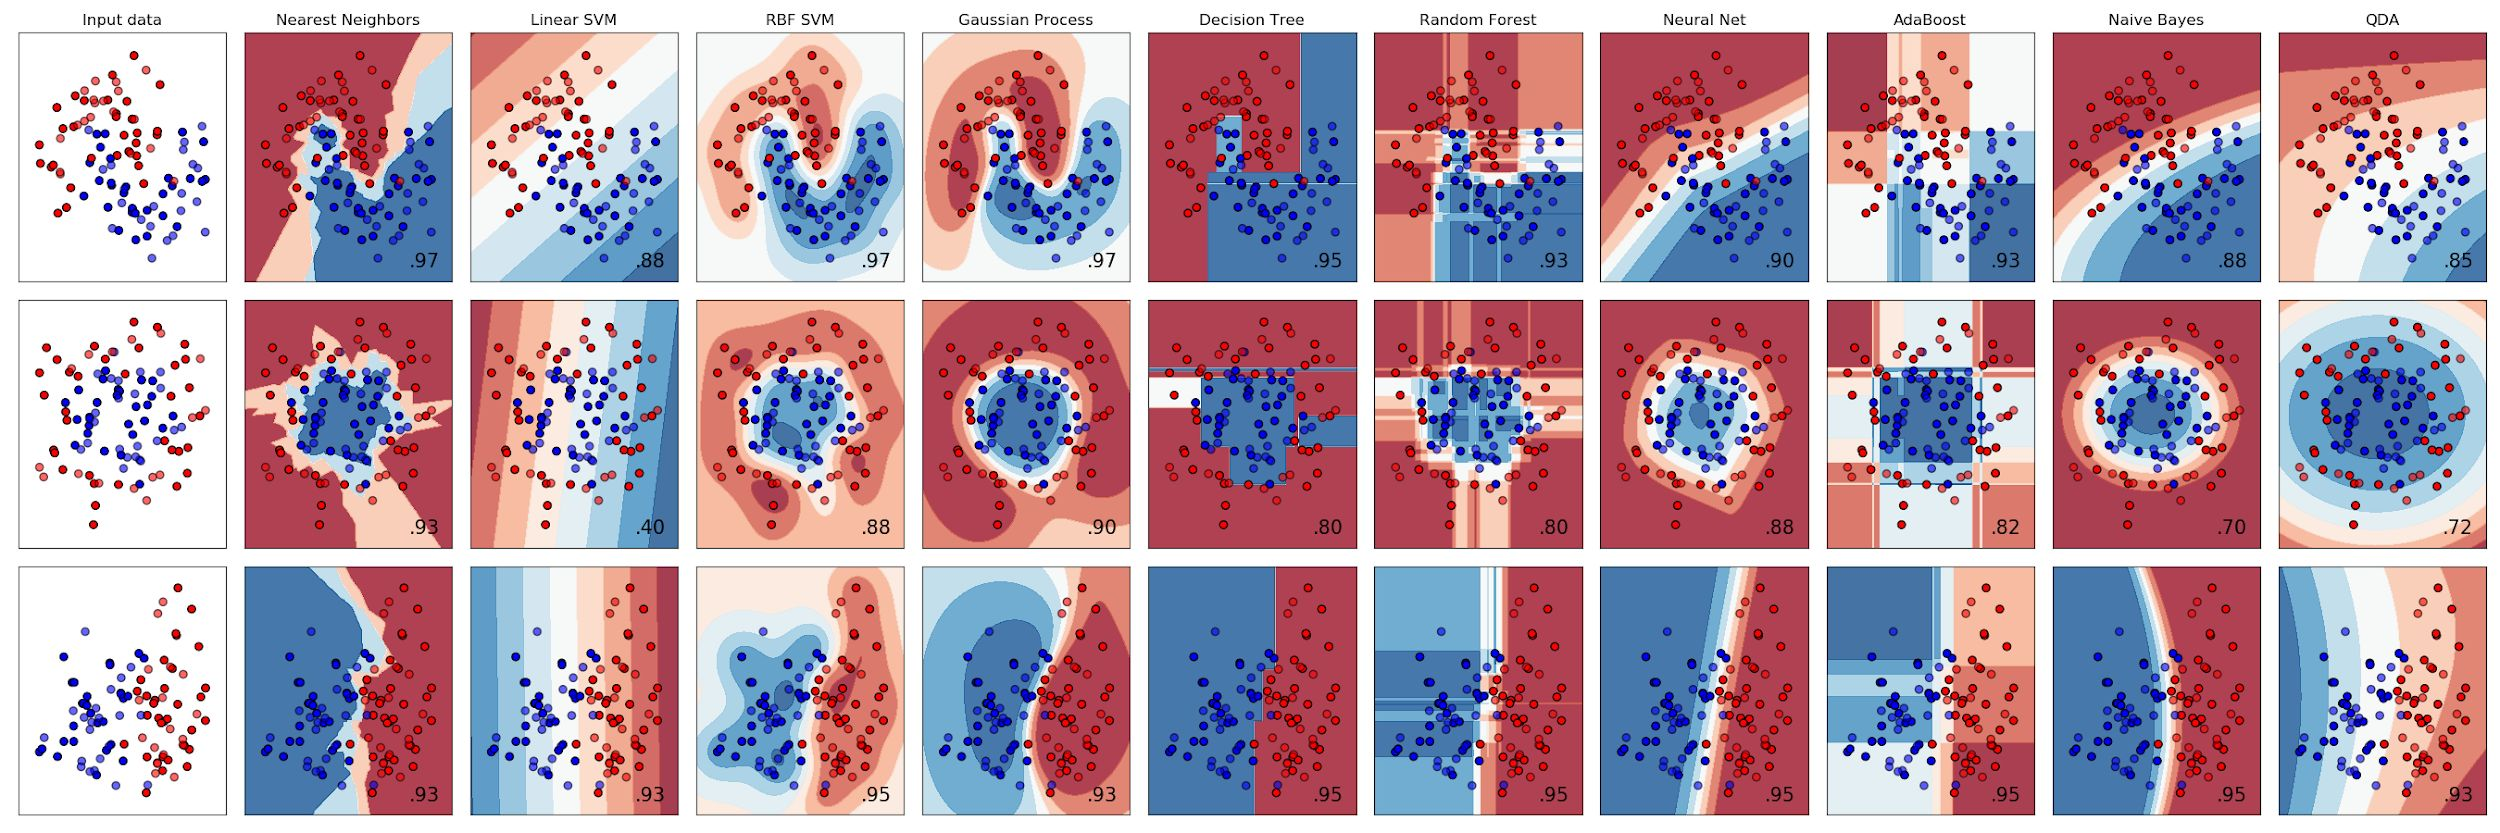
\includegraphics[width=0.9\textwidth]{figure_ml/scikit.png}
\end{figure}
\FloatBarrier

\subsection{What do we need to create our first ML program}

-Load some data
\begin{itemize}
	\item We use numpy arrays as data structures, today we load data from some existing repositories
	\item We need an “X” and a “y” array for input data and for labels (for a supervised algorithm)
	\item Different examples on the same dataset are placed in ROWS
	\begin{itemize}
		\item Rows are corresponding to the first index in numpy multi index array (aka tensor)
		\item Columns correspond to different “input features”
	\end{itemize}
\end{itemize}

-Use some existing library implementing a ML algorith (Python library exists for almost any ML algorithm).\\

-Feed the data to the library (We need to understand for each library how you run the “training” step)\\

Check the result: We need to understand how to do the inference of a trained model, for example on a new sample or on a new dataset.

\subsection{Hands-on}


First exercise is taken from \href{http://shop.oreilly.com/product/0636920034919.do}{Python Data Science Handbook} by Jake
VanderPlas with some minor edits (the content is available on \href{https://github.com/jakevdp/PythonDataScienceHandbook}{GitHub} 
Click here and “make a copy” to be able to edit: \url{https://colab.research.google.com/drive/1Sqn5fuiB5-2EP6UKUmwqjQd_b3uUNu2r?usp=sharing}\\
NB: the example uses scikit learn library, that we will NOT use in the next lectures

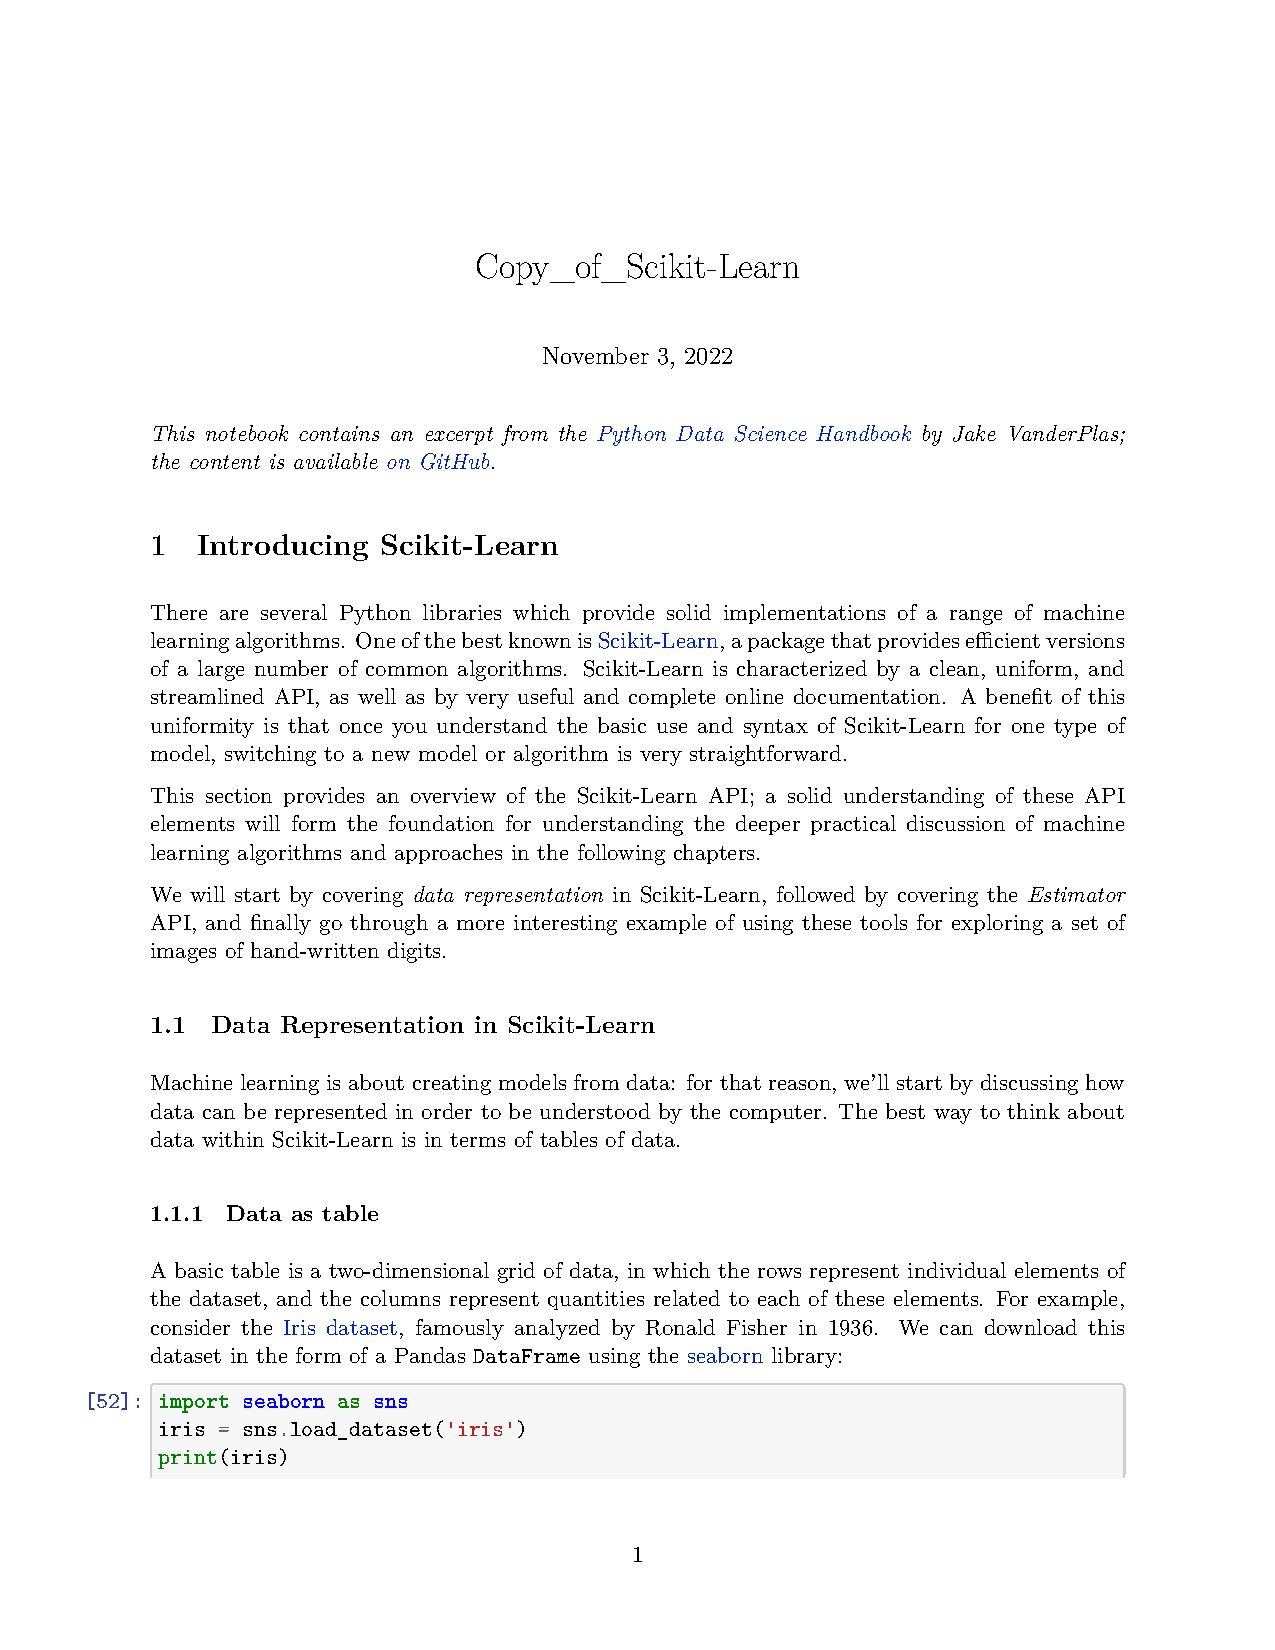
\includepdf[pages=-]{Copy_of_Scikit-Learn.pdf}
%\subsection{Python numpy reshape and stack cheatsheet}
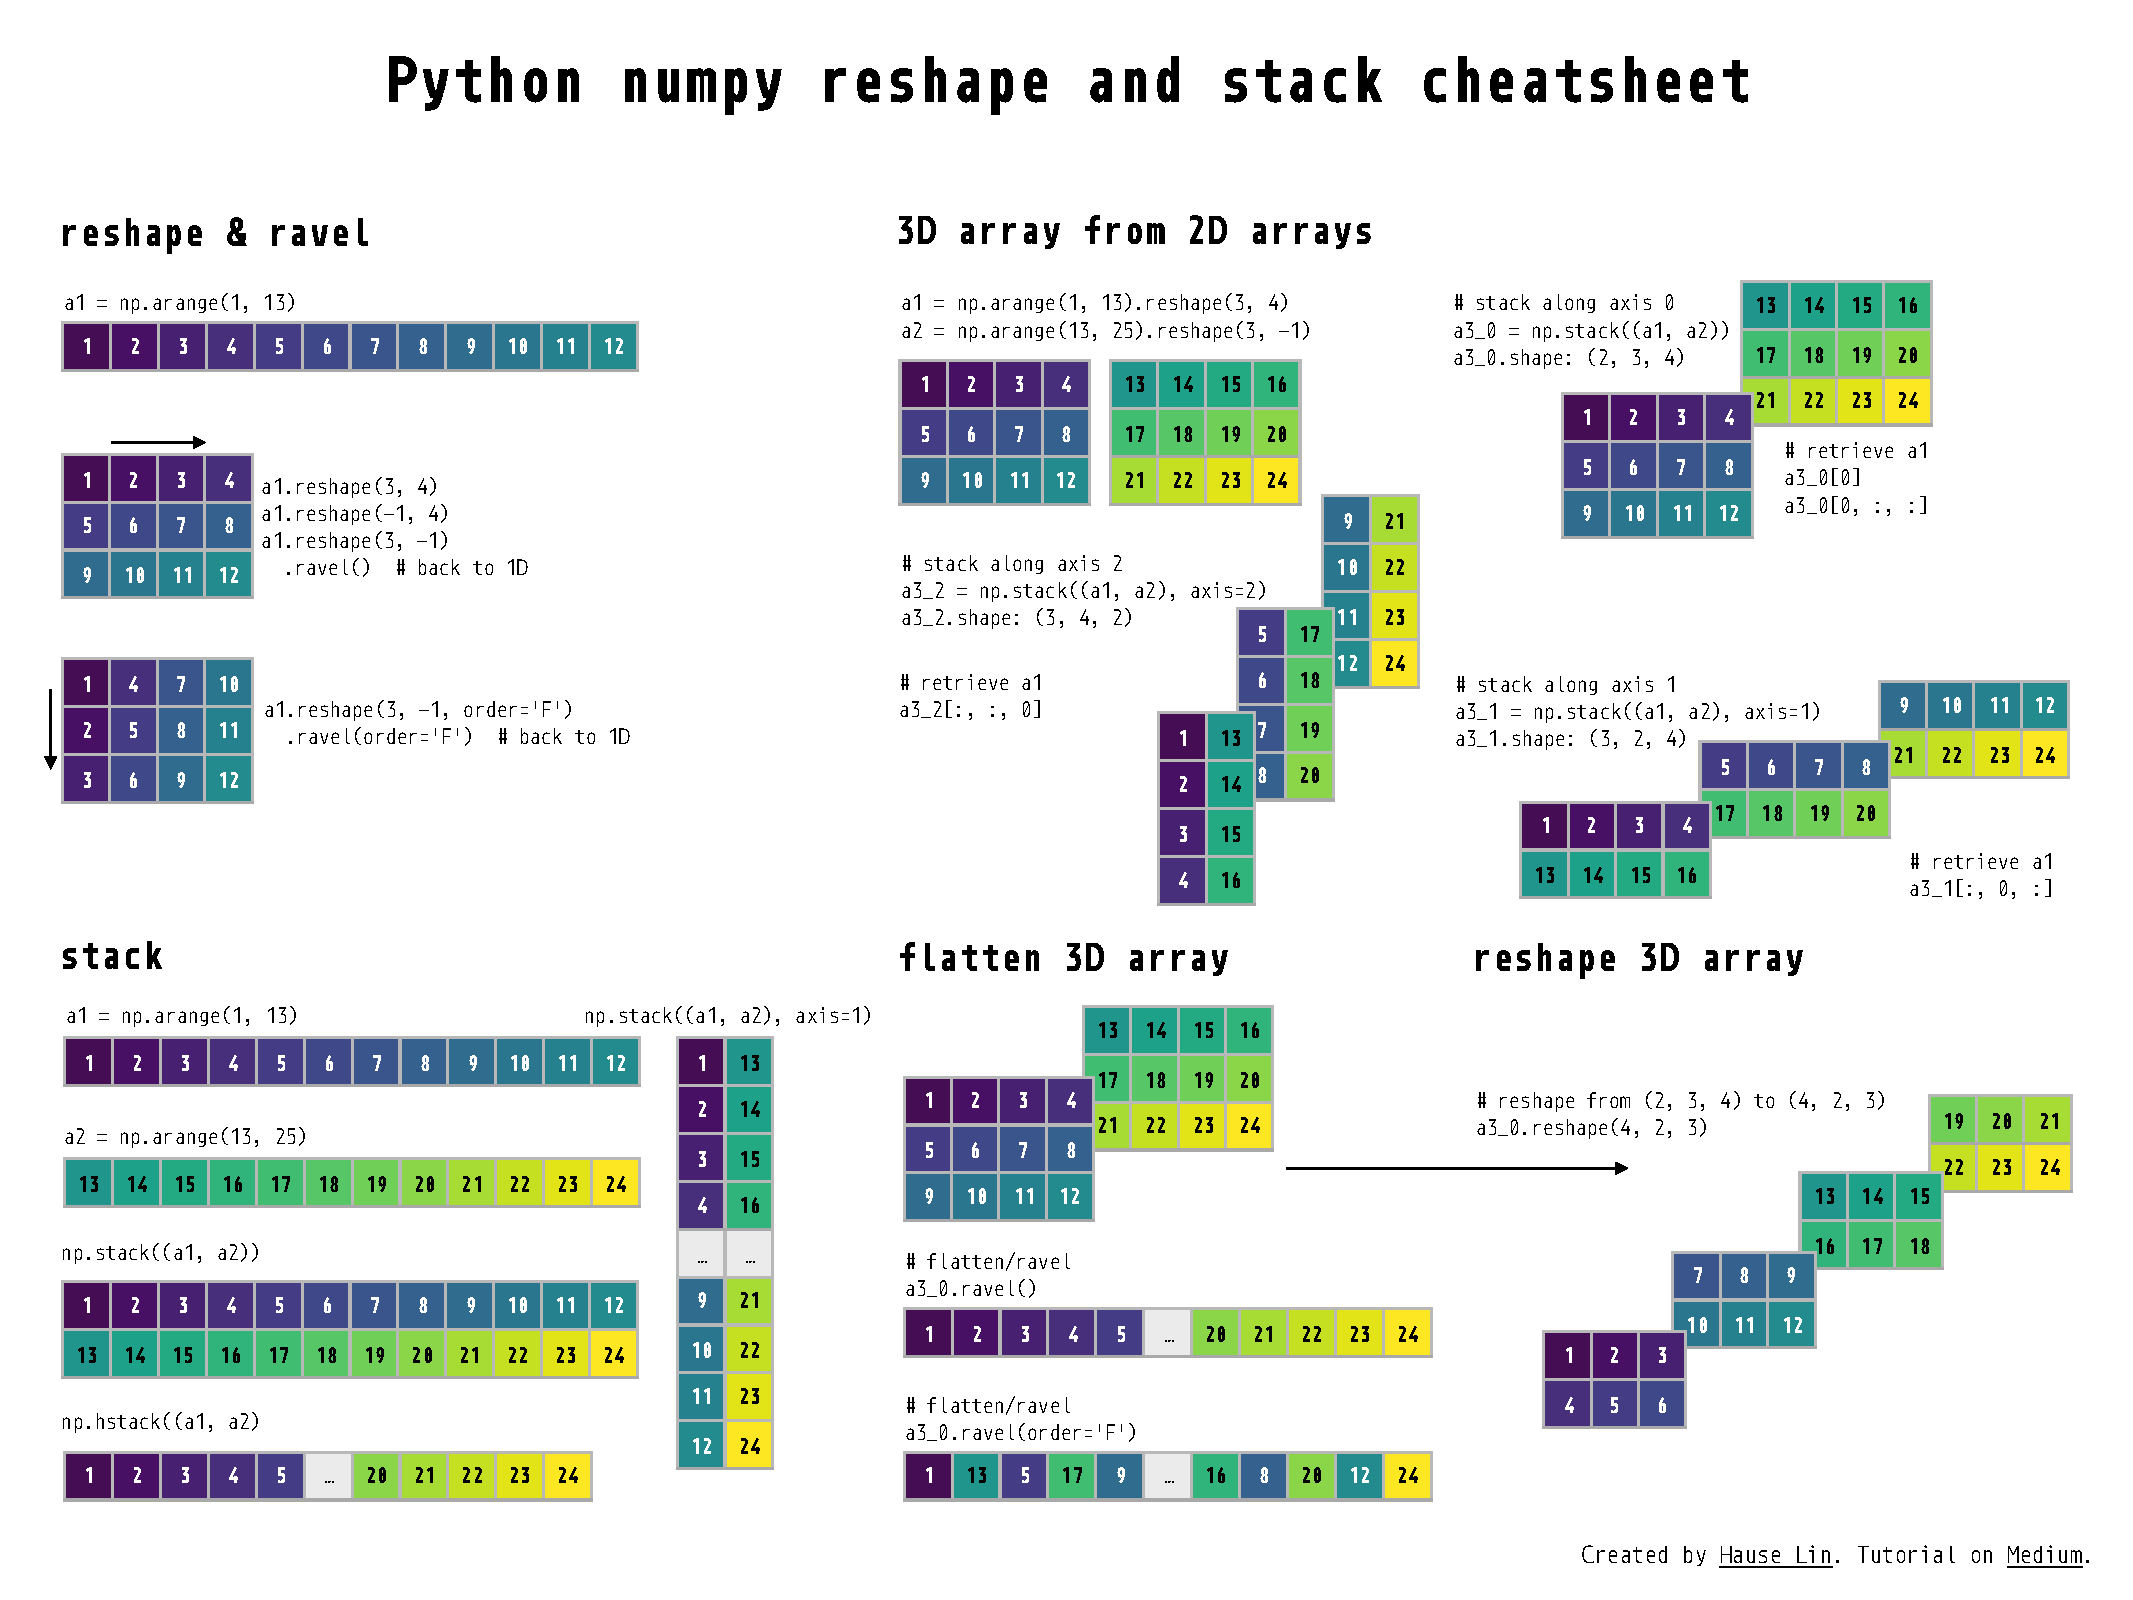
\includepdf[pages=-]{reshape.pdf}

\section{\textit{Lun 7 novembre - lezione 13}}

\section{Introduction to Artificial Neural Networks}

\begin{tcolorbox}[width=\textwidth,colback={white},title={Recap lezione 1 },colbacktitle=cyan,coltitle=black]
	\begin{itemize}
	\item ML techniques have common elements:
		\begin{itemize}
			\item The function “f” to approximate
			\item The model used to approximate “f” (e.g. polynomials functions or a decision tree or a NN)
			\item The parameters of the model (e.g. the coefficients of the poly) 
			\item The hyper-parameters of the models (e.g. the grade of the polynomial, N=1 for linear)
			\item The objective function (i.e. the loss such as MSE or binary cross entropy)
			\item The variance-bias tradeoff (aka training vs generalization)
			\item The regularization techniques
		\end{itemize}
	\item Example of ML algorithms
		\begin{itemize}
			\item Linear regression
			\item PCA
			\item Nearest Neighbours
			\item Decision trees
			\begin{itemize}
				\item Bagging vs boosting
			\end{itemize}
		\end{itemize}
	\end{itemize} 
\end{tcolorbox}

\section{Artificial Neural Networks}
\subsection{(Artificial) neural networks: the “Model”}


\begin{itemize}
	\item Computation achieved with a network of elementary computing units (neurons) 
	\item Each basic units, a neuron, has:
	\begin{itemize}
		\item \textbf{Weighted} input connections to other neurons
		\item A \textbf{non linear} activation function
		\item An output value to pass to other neurons
	\end{itemize}
	\item Biologically inspired to brain structure as a network of neuron
	\begin{itemize}
		\item But artificial NN goal is not that of “simulating” a brain!
	\end{itemize}
	\item Actual modern NN go much beyond the brain-inspired models
\end{itemize}

\begin{figure}[ht]
	\centering
	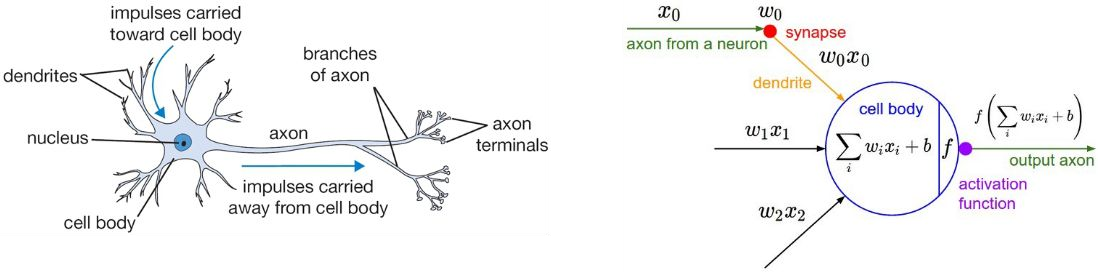
\includegraphics[width=0.9\textwidth]{figure_ml/model.png}
\end{figure}
\FloatBarrier

\subsection{Brief history, highs and lows}

\begin{wrapfigure}{r}{0.6\textwidth}
	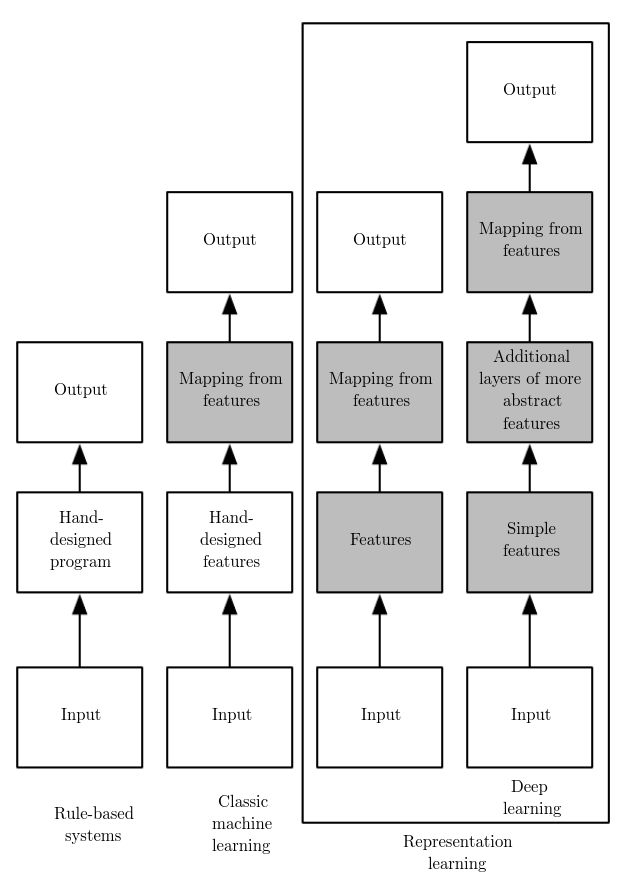
\includegraphics[width=0.6\textwidth]{figure_ml/history.png}
\end{wrapfigure} 

\quad
\begin{itemize}
	\item First work originates back in ~1940-1960 “cybernetics” 
	\begin{itemize}
		\item Linear models
	\end{itemize}
	\item Then called “connectionism” in ’80-’90
	\begin{itemize}
		\item development of neural networks, backpropagation, non-linear activations (mostly sigmoid)
	\end{itemize}
	\item High expectations, low achievements in the ‘90
	\begin{itemize}
		\item A decade of stagnation
	\end{itemize}
	\item New name, “Deep Learning”, from 2006
	\begin{itemize}
		\item Deep architectures (see next slides)
		\item Very active field in the past decade
		\item Availability of GP-GPU game changing on typical “size”
		\item Processing raw, low level, features
		\begin{itemize}
			\item It doesn’t mean you \textbf{must} use “raw features” but that rather that you \textbf{can} use raw features!
		\end{itemize}
	\end{itemize}
\end{itemize}

Dal 2006 in poi è diventato disponibile un sistema di calcolo pensato per fare videogiochi (GPU), che però si prestano bene anche al calcolo necessario per questo tipo di computing.


\subsection{Complexity growth}
Dataset become larger and larger (“big data”). Not just in “industry”, experimental scientific research is now producing multi PetaByte datasets. Digital era => everything can be “data”.\\

Increasing hardware performance => increasing complexity of the network (number of neurons and connections).\\
\begin{itemize}
	\item 2020 largest ANN: OpenAI GPT3, 175 billion parameters ( $10^{11}$)
	\item 2021 “Switch transformer” and “Wu Dao 2.0” => trillion parameters models ( $10^{12}$ )
	\item (for comparison) Human brain $10^{13} - 10^{15} $synapses ( ~ parameters )
\end{itemize}

\begin{figure}[ht]
	\centering
	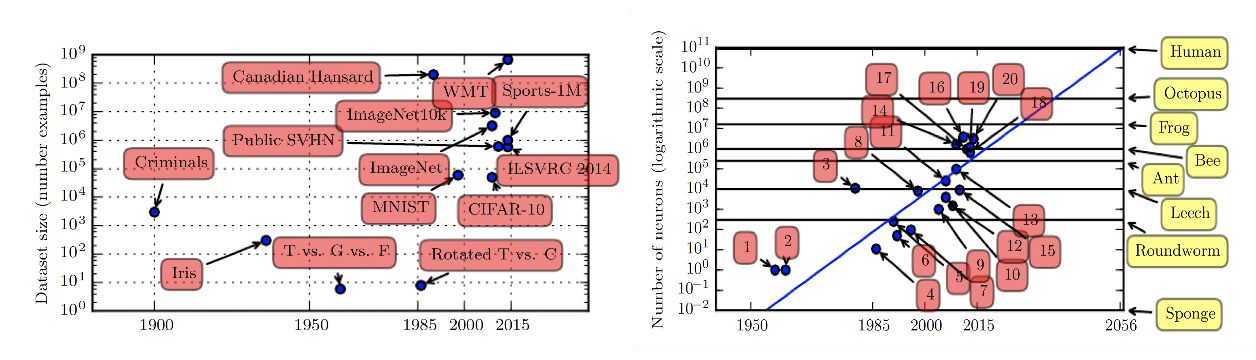
\includegraphics[width=1\textwidth]{figure_ml/complexity_growth.png}
\end{figure}
\FloatBarrier

\subsection{Performance on classic problems}
Image classification and speech recognition are the typical problems where ML (and Neural Networks) failed in the 90’. Now it beats humans...
\begin{figure}[ht]
	\centering
	\begin{subfigure}{.5\textwidth}
		\centering
		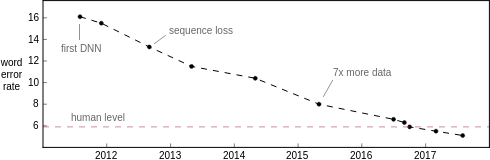
\includegraphics[width=1\linewidth]{figure_ml/speech.png}
	\end{subfigure}%
	\begin{subfigure}{.5\textwidth}
		\centering
		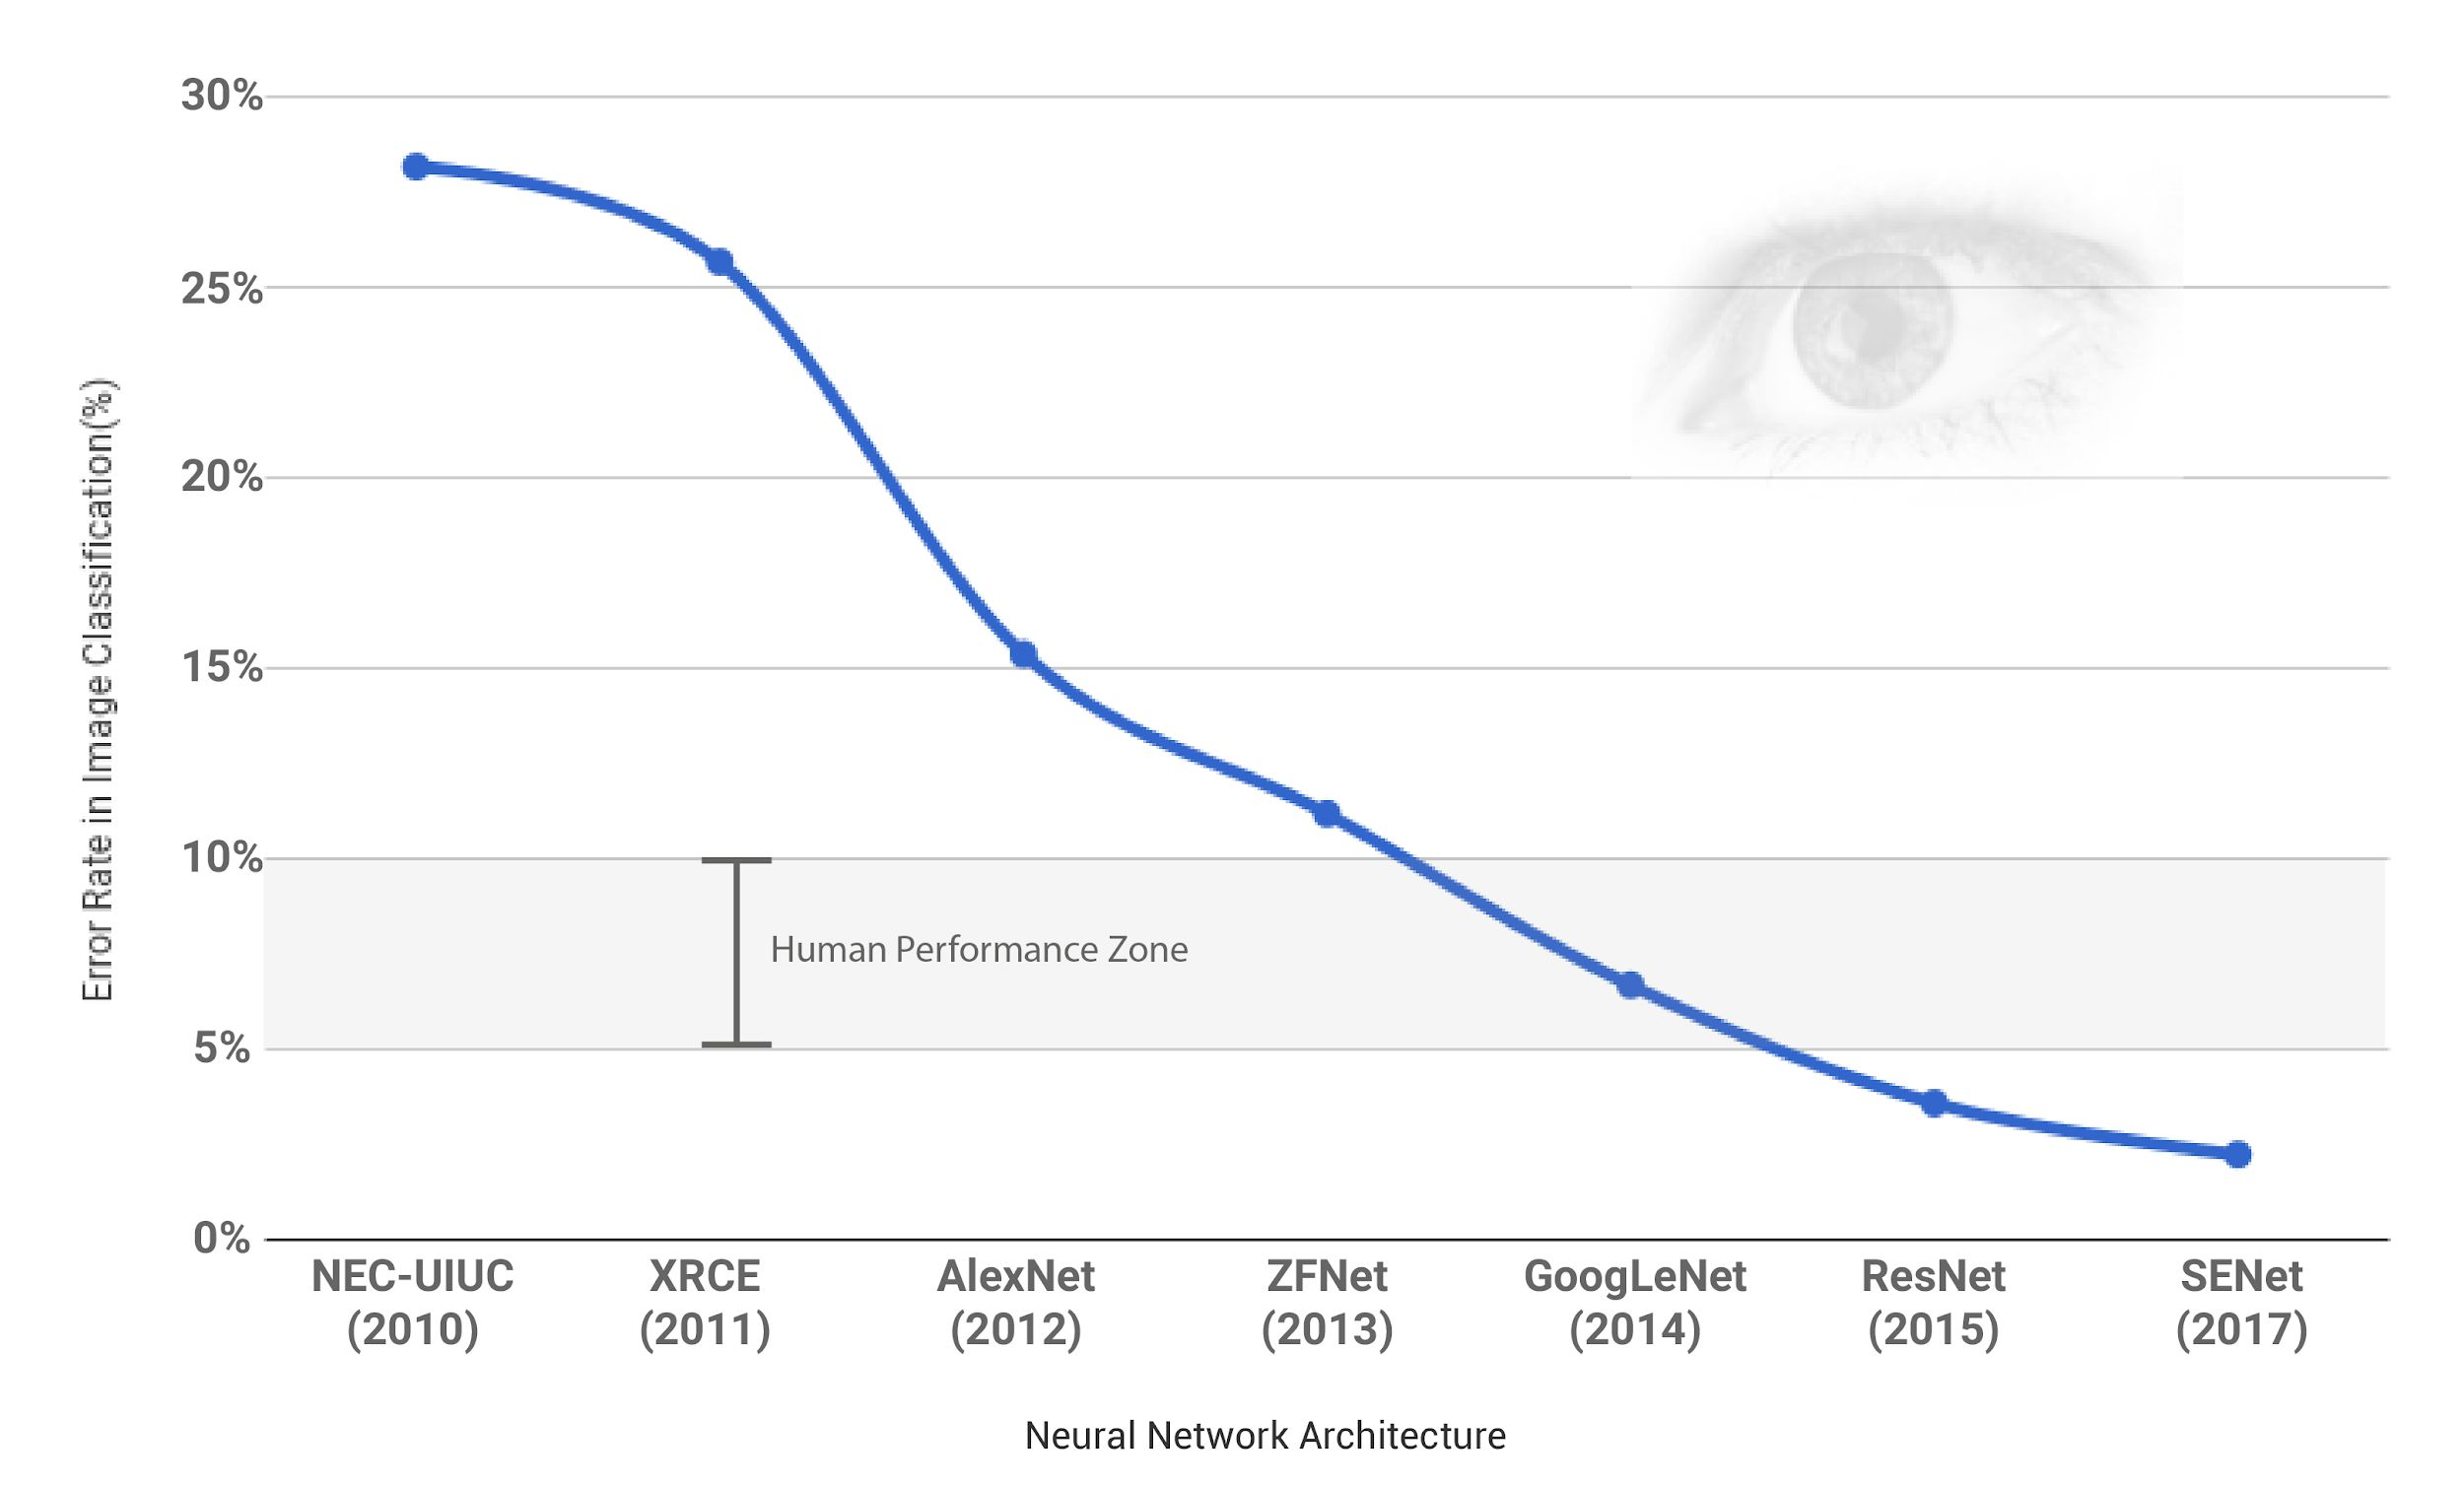
\includegraphics[width=1\linewidth]{figure_ml/img_class.png}
	\end{subfigure}
\end{figure}


\subsection{My favorite performance examples}

\begin{itemize}
	\item 
\end{itemize}

\url{https://www.technologyreview.com/2020/11/03/1011616/ai-godfather-geoffrey-hinton-deep-learning-will-do-everything/}

\subsection{OpenAI GPT3}

Generative Pre-trained Transformer A 12M\$ autocomplete (that is not really understanding what is talking about, but can still write better than most of us). \url{https://openai.com/blog/openai-api/}\\
\url{https://doi.org/10.1007/s11023-020-09548-1}.
\section{Neural Nets Basic elements}
\subsection{A neural network node: the artificial neuron}
The elementary processing unit, a neuron, can be seen as a node in a directed graph. Inputs are \textbf{summed}, with \textbf{weights}, and an \textbf{activation function} is evaluated on such sum.\\
Nodes are typically also connected (with weight b) to an input “bias node” that has a fixed output value of 1. Different activation functions can be used, common ones are: sigmoid, atan, relu (rectified linear unit).

\begin{figure}[ht]
		\centering
		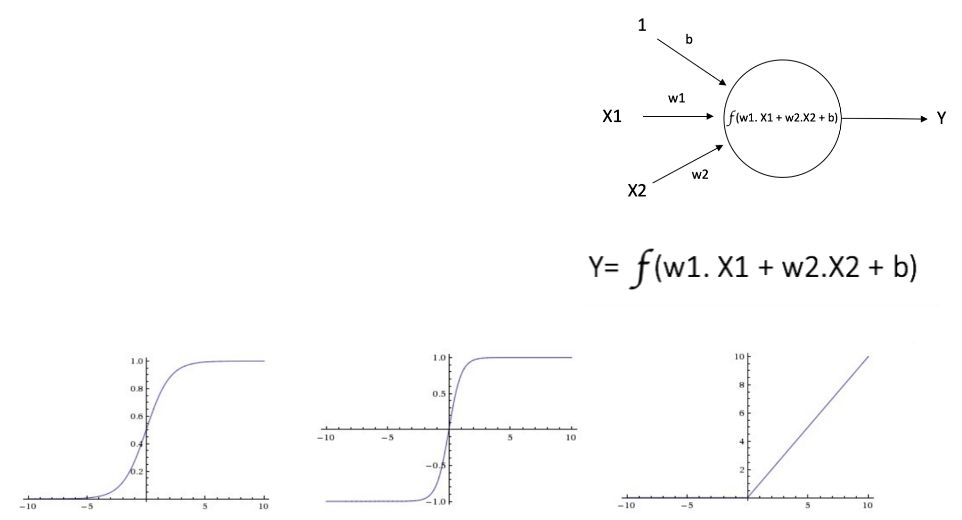
\includegraphics[width=0.7\linewidth]{figure_ml/neuron.png}
\end{figure}
\FloatBarrier


\subsection{The MLP model}

\begin{wrapfigure}{r}{0.6\textwidth}
	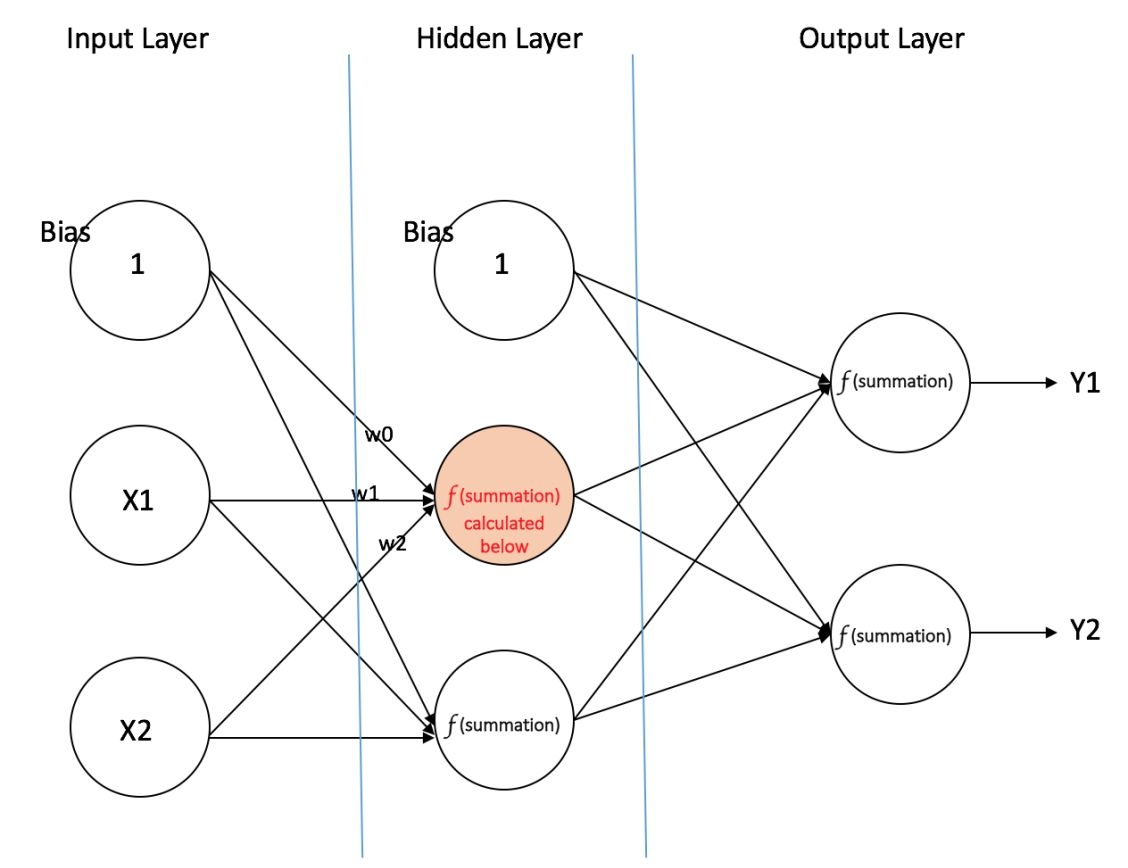
\includegraphics[width=0.6\textwidth]{figure_ml/mlp.png}
\end{wrapfigure} 
\quad
\begin{itemize}
	\item The most common NN in the ‘90 was the Multi Layer	Perceptron (MLP)
	\item Graph structure organized in “layers”
		\begin{itemize}
			\item Input layer (nodes filled with input value)
			\item Hidden layer
			\item Output layer (node(s) where output is read out)
		\end{itemize}
	\item Nodes are connected only from one layer to the next and all possible connections are present (known as \textbf{“dense” or “fully connected”} layer)
		\begin{itemize}
			\item No intra-layer connections
			\item No direct connections from input to output
		\end{itemize}
	\item Size of input and output layers are fixed by the problem
	\item \textbf{Hyperparameters} are
		\begin{itemize}
			\item The size of the hidden layers
			\item The type of activation function
		\end{itemize}
	\item The \textbf{parameters} to learn are the weights of the connections
\end{itemize}

\subsection{Universal approximation theorem}
\textit{“One hidden layer is enough to represent (not learn) an approximation of any function to an arbitrary degree of accuracy”} (I. Goodfellow et al. 2016).\\

\begin{itemize}
	\item You can approximate any function with arbitrary precision having \textbf{enough hidden nodes} and the \textbf{right weights}
	\item How do you get the right weights? You need a “training” for your network
	\begin{itemize}
		\item The theorem does not say that one hidden layer (+ some training algorithm) is enough to find the optimal weights, just that they exists!
	\end{itemize}
	\item Achieving some (even modest with some metric) level of accuracy may need an unmanageable hidden layer size
	\begin{itemize}
		\item And may need an unreasonable number of “examples” to learn from
	\end{itemize}
\end{itemize}

\subsection{Example (1-D input)}

\begin{figure}[ht]
	\centering
	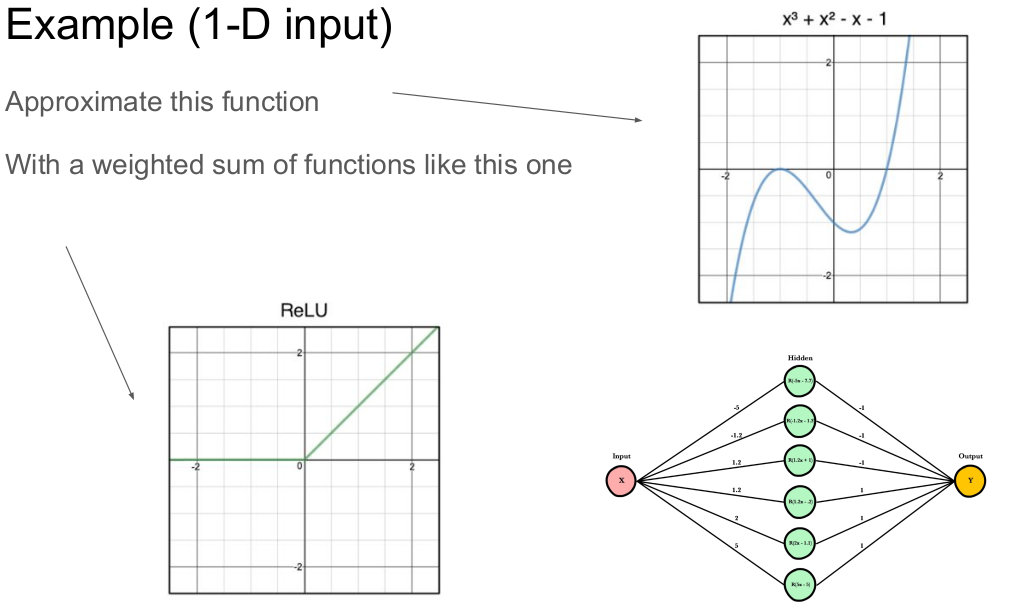
\includegraphics[width=0.9\linewidth]{figure_ml/example1d.png}
\end{figure}
\FloatBarrier

The Universal Approximation Theorem says that increasing \#nodes I can
increase the accuracy as much as I want. More hidden nodes, higher “capacity” => more accuracy

\begin{figure}[ht]
	\centering
	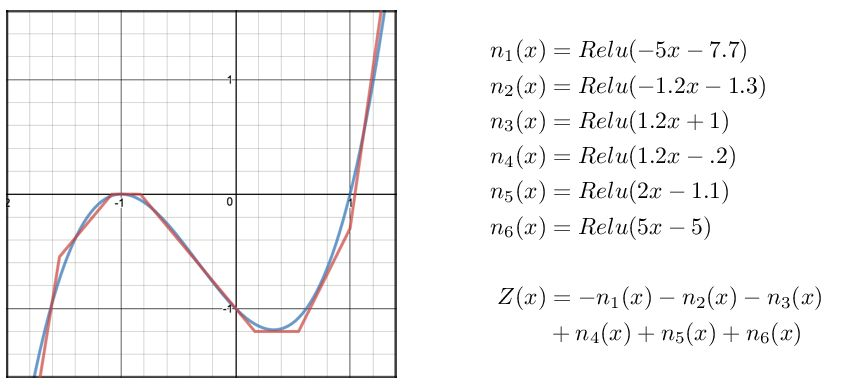
\includegraphics[width=0.7\linewidth]{figure_ml/example1d2.png}
	\caption{\url{https://towardsdatascience.com/can-neural-networks-really-learn-any-function-65e106617fc6}}
\end{figure}
\FloatBarrier

\subsection{Training of an MLP}
How do I get the weights?\\
Remember: we do not know the function we want to approximate, we only have some “samples”.

\begin{figure}[ht]
	\centering
	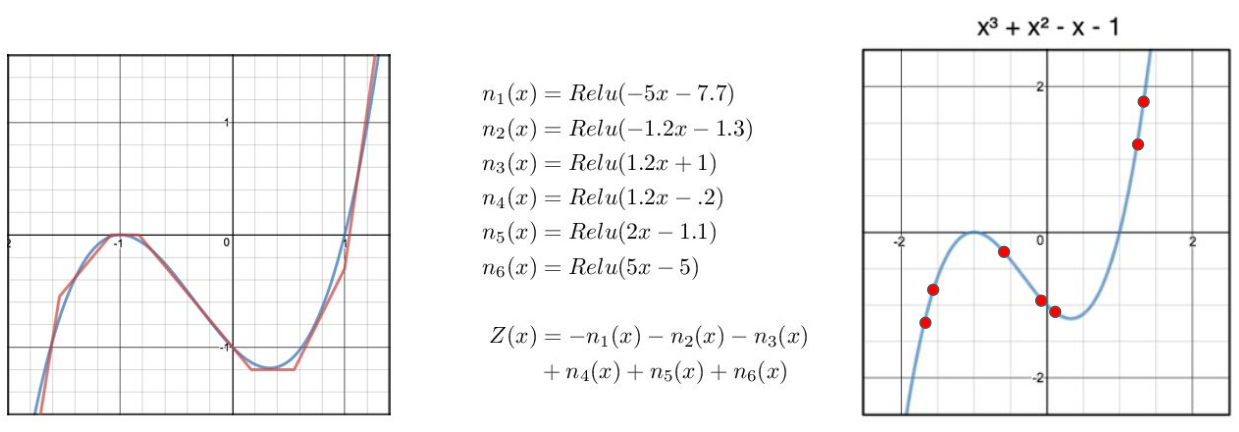
\includegraphics[width=0.9\linewidth]{figure_ml/training_mlp.png}
\end{figure}
\FloatBarrier

\subsection{Training a NN}


\begin{wrapfigure}{r}{0.4\textwidth}
	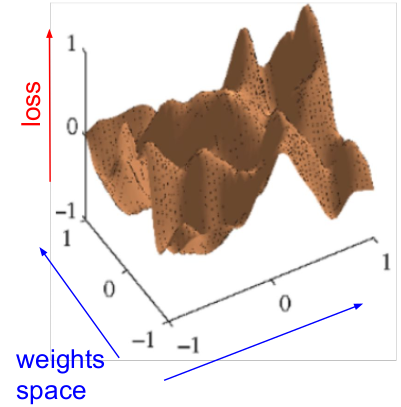
\includegraphics[width=0.4\textwidth]{figure_ml/training_nn.png}
\end{wrapfigure} 

The goal of training is to minimize the objective
function (possibly both on the training and validation
sample). I.e. we want to minimize the loss as a function of the model parameters (i.e. the weights).\\
For a MLP the basic idea is the following


\begin{enumerate}
	\item Start with random weights
	\item Compute the prediction y\_pred for a given input x and compare target y\_true computing the loss (repeat for a few example, aka “one batch”)
	\item Estimate an update for the weights that reduces the loss
	\item Iterate from point (b), repeating for all samples
	\item When the sample has been used completely (end of an epoch), iterate from (b) again on all samples
	\item Repeat for multiple epochs
\end{enumerate}

The important point is how to implement point (c) => (stochastic) gradient descent.

\subsection{How to find a minimum?}


\begin{wrapfigure}{r}{0.4\textwidth}
	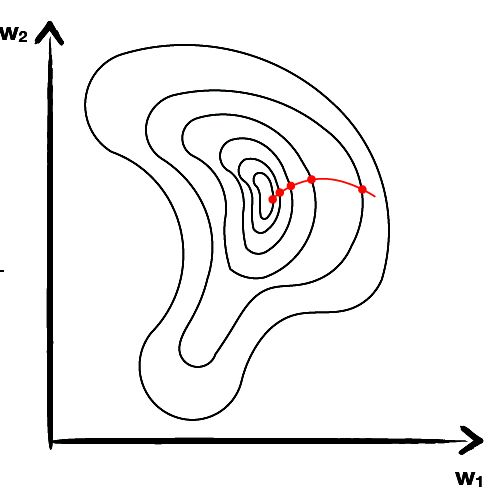
\includegraphics[width=0.4\textwidth]{figure_ml/find_minimum.png}
\end{wrapfigure} 

\textbf{Gradient Descent}\\
We know the loss function value in a point in the weights phase space (e.g. the initial set of random weights, or the iteration
N-1), computed numerically as the mean or the sum of the losses for each of our training examples.\\
We can compute the gradient of the loss function in that point, we expect the minimum on “the way down” hence we adjust our set of weights doing a “step” in the direction pointed by the gradient with a step size that is proportional to the length
of the gradient.\\

\textbf{Stochastic Gradient Descent (SGD):}
Compute the gradient on “batches” of events rather than full sample. The “noise” may help avoiding local minima.

\subsection{Not as simple as you would imagine}

A parameter named \textbf{learning rate} controls how big the step in the direction of the gradient is.
\begin{itemize}
	\item A too large step may let you bounce back and forth on the walls of your “valley”
	\item A too small step would make your descent lasting forever
\end{itemize}
Several variants of SGD
\begin{itemize}
	\item Include “momentum” from previous gradient	calculations (may help overcome local obstacles) 
	\item Reduce step size over time
	\item Adadelta, Adagrad, \textbf{Adam}, and many more
\end{itemize}


\begin{figure}[ht]
	\centering
	\begin{subfigure}{.5\textwidth}
		\centering
		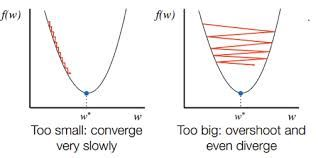
\includegraphics[width=1\linewidth]{figure_ml/sgd.png}
	\end{subfigure}%
	\begin{subfigure}{.4\textwidth}
		\centering
		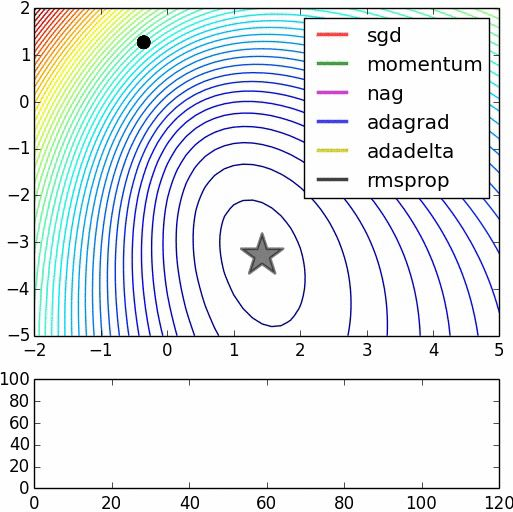
\includegraphics[width=1\linewidth]{figure_ml/sgd2.png}
	\end{subfigure}
\end{figure}



\subsection{Learning rate, epochs and batches}


\begin{wrapfigure}{r}{0.35\textwidth}
	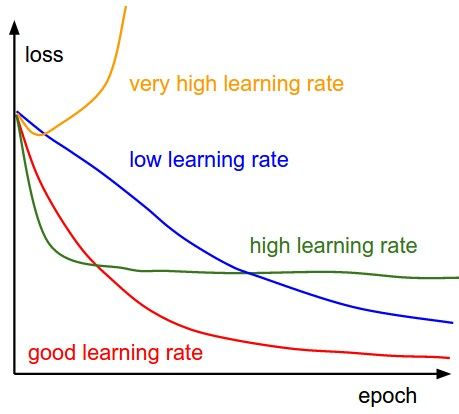
\includegraphics[width=0.35\textwidth]{figure_ml/learning_rate.png}
\end{wrapfigure} 

The gradient update (in SGD) is repeated for each “batch” of events.\\

A full pass of the whole dataset (i.e. all batches) is called an epoch.\\

A typical training foresee iteration on multiple epochs.\\

The size of the update step can be controlled with a multiplicative factor called “learning rate”. Learning rate can be adapted over time.

\begin{figure}[ht]
	\centering
	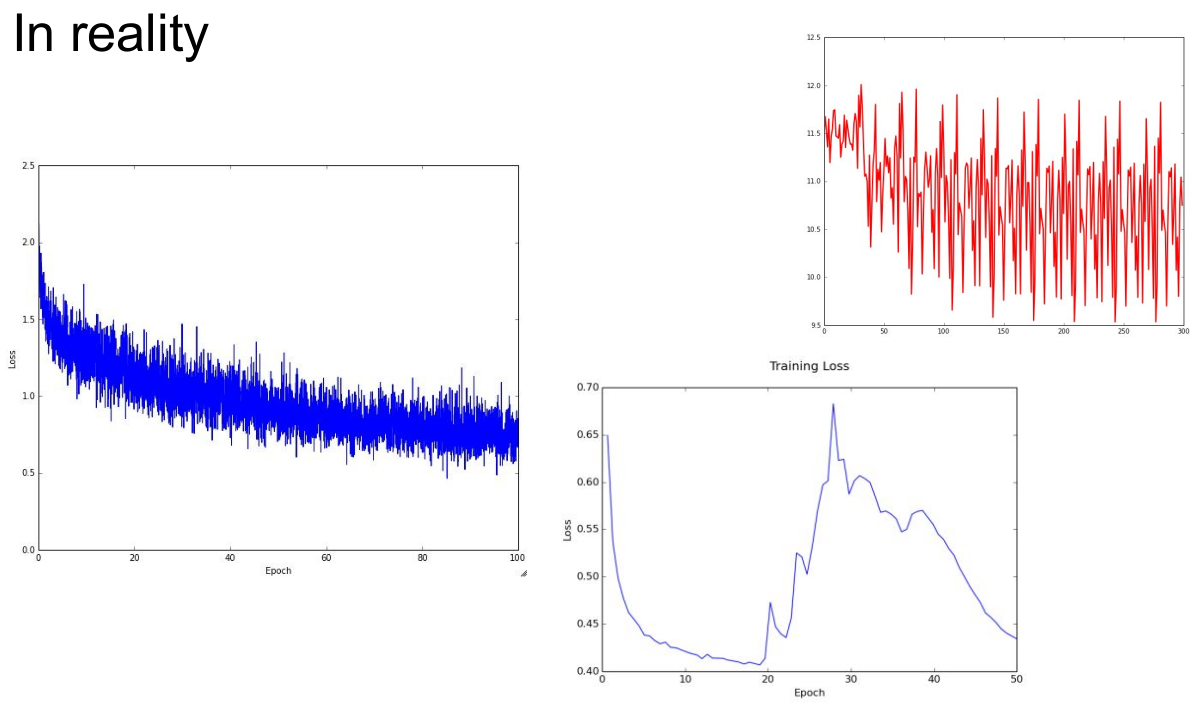
\includegraphics[width=0.8\linewidth]{figure_ml/real_lr.png}
\end{figure}
\FloatBarrier

\clearpage
\subsection{Training and overfitting}

\begin{wrapfigure}{r}{0.35\textwidth}
	\includegraphics[width=0.35\textwidth]{figure_ml/training_overfitting.png}
\end{wrapfigure} 
As discussed previously if the capacity is large enough the network could “overfit” on the training dataset.

\begin{itemize}
	\item Have a separate, stat independent, validation/generalization sample
	\item Evaluate performance (with “loss” or with other metrics) on the validation sample
	\item Training results depends on many choices
	\begin{itemize}
		\item Size of batches (amount of “noise”)
		\item Learning rate (how much you move along the gradient at
		each iteration)
		\item Gradient Descent algorithm
		\item Capacity of the network
	\end{itemize}
\end{itemize}

\subsection{Neural Networks, computers and mathematics}
ANN use a fairly limited and simple set of operations
\begin{itemize}
	\item Many operation are simply represented with linear algebra
	\item Non linear function are typically applied, repeated, to multiple inputs (hence can be “vectorized”)
	\item Gradient Descent works by knowing the derivatives of the functions involved in the NN calculations (weights, activations) and in the loss
\end{itemize}

Datasets are represented as multidimensional tensors

\begin{itemize}
	\item The number of indices and the length per index is usually called “shape” and is a tuple with dimension of each index
	\item The first index is the one running the “number of sample in the dataset”, and is sometimes omitted when describing a neural network
\end{itemize}

Classification with multiple category is often converted in the “categorical” representation
\begin{itemize}
	\item I.e. rather than labelling with a scalar “y” (with 0=horse, 1=dog, 2=cat, 3=bird, …) a vector y is used with as many components as the category (with [1,0,0,0]=horse, [0,1,0,0]=dog, etc..)
\end{itemize}
Tools exist to describe mathematically the network structure that are optimized for fast computations on CPU/GPU/TPU
\subsection{Back-propagation}

\begin{figure}[ht]
	\centering
	\includegraphics[width=1\linewidth]{figure_ml/backpropagation.png}
\end{figure}
\FloatBarrier


\section{Deep Networks}

\subsection{Deep Feed Forward networks}

\begin{figure}[ht]
	\centering
	\includegraphics[width=1\linewidth]{figure_ml/activation_functions.png}
\end{figure}
\FloatBarrier


\subsection{Why going deeper?}
Hold on… wasn’t there a theorem saying that MLP is good enough ? Yes but…
\begin{itemize}
	\item Amount of nodes to represent complex functions can be too high
	\item Learning the weights on finite samples could be too difficult
\end{itemize}

Advantages of Deep architectures

\begin{itemize}
	\item Hierarchical structure can allow easier “abstraction” by the network with early layers computing low level features and deeper layers representing more abstract properties 
	\item Number of neurons and connections needed to represent the same function highly reduced in many realistic cases
\end{itemize}
I primi layer imparano features più semplici, quelli dopo imparano features sempre di più alto livello.

\subsection{Activation functions}
\begin{figure}[ht]
	\centering
	\includegraphics[width=1\linewidth]{figure_ml/activation_functions.png}
\end{figure}
\FloatBarrier

\newpage
\subsection{Deep architectures}

\begin{figure}[ht]
	\centering
	\includegraphics[width=0.85\linewidth]{figure_ml/mcc_NN}
\end{figure}
\FloatBarrier

\newpage

\subsection{Dropout and regularization methods}

NN training is a numerical process. Often the number of samples is limited hence the gradient accuracy is not great. Several regularization methods exists to avoid being dominated by stochastic effects.
\begin{itemize}
	\item Caps to the weights (so that individual nodes cannot be worth more than some amount)
	\item \textbf{Dropout} techniques: during the training a fraction of nodes
	is discarded, randomly, at each iteration
	\begin{itemize}
		\item NN more robust to noise
		\item Effectively “augmenting” the input dataset
	\end{itemize}
\end{itemize}


\begin{figure}[ht]
	\centering
	\includegraphics[width=0.5\linewidth]{figure_ml/dropout.png}
\end{figure}


\subsection{(Batch) normalization}
Input features have typically different ranges, means, variance.\\
It is generally useful to “normalize” the input distribution:
\begin{itemize}
	\item Mean zero
	\item Variance 1
\end{itemize}

Often it could be practical to compute the normalization on individual batches rather than full sample (Batch vs full sample ? may depend on your use case).

\begin{figure}[ht]
	\centering
	\includegraphics[width=0.8\linewidth]{figure_ml/batch_norm.png}
\end{figure}
\FloatBarrier

\section{DNN Tools}


\subsection{Keras}

Keras is a python library that allow to build, train and evaluate NN with many modern technologies.\\
Keras supports multiple backends for actual calculations.\\
Two different syntax are usable to build the network architecture
\begin{itemize}
	\item Sequential: simple linear “stack” of layers
	\item Model (functional API): create more complex topologies
\end{itemize}

Multiple type of “Layers” are supported

\begin{itemize}
	\item Dense: the classic fully connected layer of a FF network
	\item Convolutional layers
	\item Recurrent layers
\end{itemize}

Multiple type of activation functions.\\
Various optimizers and gradient descent techniques.

\subsection{Other common tools}

Common alternative to keras

\begin{itemize}
	\item Pytorch (trending up!) 
	\item Sonnet 
	\item Direct usage of TensorFlow (or other backends, e.g. Theano)
	\begin{itemize}
		\item Need to write yourself some of the basics of NN training
		\item Especially useful to develop new ideas (e.g. a new descent technique, a new type of basic unit/layer)
	\end{itemize}
\end{itemize}

\subsection{Keras Sequential example}

\begin{figure}[ht]
	\centering
	\includegraphics[width=0.8\linewidth]{figure_ml/seq_ex.png}
\end{figure}
\FloatBarrier
\subsection{Keras “Model” Functional API}


\section{Keras Layers}
\subsection{Keras basic layers}

\begin{itemize}
	\item 
\end{itemize}


%finire lez 2

\section{\textit{Giovedì 10 novembre - Lezione 14}}

\section{Convolutional and recurrent networks}

\subsection{Classification of images}

Come si fa a processare un'immagine con una rete neurale?\\

\begin{figure}[ht]
	\centering
	\includegraphics[width=0.3\linewidth]{figure_ml/classif.png}
\end{figure}
\FloatBarrier

Images are data structure with 2 or 3 indices: X,Y or X,Y,channel (=R,G,B)
\begin{itemize}
	\item Shape of the input dataset (Nsamples, Width, Height, nchannels)
	\item nchannels is typically 1 (B\&W), 3 (RGB) or 4 with transparency
\end{itemize}
We can use FF networks to classify images
\begin{itemize}
	\item Reshape the input tensor with the “Flatten” keras layer
\begin{figure}[ht]
	\centering
	\begin{subfigure}{.3\textwidth}
		\centering
		\includegraphics[width=0.9\linewidth]{figure_ml/classif1.png}
	\end{subfigure}%
	\begin{subfigure}{.3\textwidth}
		\centering
		\includegraphics[width=0.9\linewidth]{figure_ml/classif2.png}
	\end{subfigure}%
	\begin{subfigure}{.3\textwidth}
		\centering
		\includegraphics[width=0.9\linewidth]{figure_ml/classif3.png}
	\end{subfigure}
\end{figure}

	
	\item Use multiple dense layers with a final one for one-hot encoding output
\end{itemize}
Limitations of this approach:
\begin{itemize}
	\item If the image is translated, even by a single pixel in x or y, the network may not recognize as “similar” to the untranslated image
	\item Nearby pixels in “Y” (or even the same pixel but in a different color) are not treated any differently than far away pixels
\end{itemize}
We know that our problem has some invariance. We know that input data has some locality information.

\subsection{Exploit invariance and locality}

\begin{wrapfigure}{r}{0.3\textwidth}
	\includegraphics[width=0.3\textwidth]{figure_ml/windows.png}
\end{wrapfigure} 
\quad
\begin{itemize}
	\item Suppose you want to count windows in a 800x600	picture with houses
	\begin{itemize}
		\item With an MLP or DFF you have 800x600x3(RGB)=1.4M inputs
		\item Each node process independently some part of the image
		\item The initial “Dense” connection should converge to something with lot of “zero” weights because far away pixel points have no reason to be considered at the same time in order to detect	local features
		\item => the problem cannot be managed this way
	\end{itemize}
\end{itemize}

But the problem is translation invariant!

\begin{itemize}
	\item “Windows” are local features, you can just analyze a patch of the image \textbf{(locality)}
	\item A window is a window no matter if it is top left or bottom right of	your image (\textbf{Invariance)}
	\item And actually windows are made of even more local features (some borders/frame, some uniform area, a squared shape)
\end{itemize}

\subsection{Can we exploit problem invariance?}

Convolutional neural networks (CNN) attempt to exploit invariance against spatial translations.
\begin{itemize}
	\item Smaller networks (locality !)
	\item Acting on a single patch of the image
	\item Stacking multiple such Convolutional Layers one after the other
	\item Use “subsampling” layer to scale from local to global
\end{itemize}

Hierarchical approach

\begin{itemize}
	\item Early layers learn local features
	\item Subsampling reduce the information extracted from a given “patch”
	\item A final flatten+one or more dense layers is used to reach the final target
\end{itemize}

\begin{figure}[ht]
	\centering
	\includegraphics[width=0.8\linewidth]{figure_ml/cnn.png}
\end{figure}
\FloatBarrier

Il vantaggio di questo approccio è che ognuna delle reti che alleniamo vedrà un numero di input molto maggiore, dato che da ogni immagine prendiamo più subsample.


\subsection{Limitations}

The linear algebra formalism we use can handle nicely images, hence implement nicely CNN (translation invariance along x and y).\\

There are more invariances out there! (Rotation, Scale, Luminosity).\\

So currently the networks have to learn them all.\\
We can do tricks to increase the number of samples in our datasets with augmentation techniques (i.e. apply random transformations of scale, rotation etc..).\\
“Built-in” invariance (such as the x-y one) has the advantage of reducing by orders of magnitude the number of weights to learn.

\subsection{Understanding the dimensions of the convolution}

\begin{itemize}
	\item Convolution can be 1D, 2D, 3D
	\item Kernel size, typically square (MxM) with M odd (but can be any shape)
	\item Padding: how to we handle borders? We can do only “valid” windows (no padding) or process borders as if there were zeros (or other values) outside
	\item Each “point” in the 1D, 2D, 3D matrix can have multiple features (e.g. R,G,B)
	\item Each Convolutional layer have mutiple outputs (filters) for every “patch” it scans on (one optimized to detect if the patch is uniformly filled, one looking for vertical lines, etc..)
\end{itemize}

\begin{figure}[ht]
	\centering
	\includegraphics[width=0.8\linewidth]{figure_ml/convolution.png}
\end{figure}
\FloatBarrier

Stride: di quanto sposto il kernel ad ogni iterazione? Posso spostarmi di 1 (ho overlap), oppure mi sposto della kernel size, o della metà etc.




\subsection{Pooling (subsampling)}

 \begin{wrapfigure}{r}{0.4\textwidth}
 	\includegraphics[width=0.4\textwidth]{figure_ml/pooling.png}
 \end{wrapfigure}

Pooling layers are simply finding maxima or computing average in patches of some convolution layer output.\\
Pooling is used to reduce the space dimensionality after a convolutional layer.
\begin{itemize}
	\item The Conv “filters” look for features (e.g. a filter may look for cats eyes)
	\item The Pooling layer checks if in a given 	region some filtered fired (there was a cat eye somewhere in this broader region)
\end{itemize}

\subsection{Typical CNN architecture}

\begin{figure}[ht]
	\centering
	\includegraphics[width=1\linewidth]{figure_ml/cnn_arch.png}
\end{figure}
\FloatBarrier

\subsection{More on convolution}


Convolution is a way to correlate \textbf{local} input information and to reduce the NN size by sharing the weights of the nodes across all repeated patches.\\

What if I have multiple objects, with no local correlation, but with multiple features (like R,G,B channels) and I want to process them all in the same way?
\begin{itemize}
	\item 1x1 convolution!
	\item Conv1D is usually enough (as the x-y coordinates have no meanin here)
	\item The symmetry here is that all “objects” are the same
\end{itemize}

\begin{figure}[ht]
	\centering
	\includegraphics[width=0.3\linewidth]{figure_ml/more_conv.png}
\end{figure}
\FloatBarrier

\textbf{Example :} Particles in a detector with information about 4-vector, tracking hits, calorimeter deposits, p-ID etc… and want to preprocess them one by one before using them for some higher level task


\subsection{Bounding Box}

 \begin{wrapfigure}{r}{0.4\textwidth}
	\includegraphics[width=0.35\textwidth]{figure_ml/stop_bb.png}
\end{wrapfigure}

In order to predict “where” an object is a “bounding box” is defined.
\begin{itemize}
	\item Coordinates of two opposite corners
	\item Essentially a “regression” problem
\end{itemize}

Not simple to extend to multiple objects in a single image, YOLO (You Only Look Once) algorithm is an option \url{https://pjreddie.com/darknet/yolo/}\\
\begin{itemize}
	\item Divide the image in cells, in each cell you predict up to N bounding box corners (relative to the cell position) 
	\item Pick only cells with high score (and cluster multiple predictions of the same bb)
\end{itemize}

\begin{figure}[ht]
	\centering
	\includegraphics[width=0.9\linewidth]{figure_ml/bb.png}
\end{figure}
\FloatBarrier


\subsection{Transfer learning}

\begin{wrapfigure}{r}{0.5\textwidth}
	\includegraphics[width=0.48\textwidth]{figure_ml/tl.png}
\end{wrapfigure}

If learn to process images of a given size, can we apply that to different size.
\begin{itemize}
	\item If the “scale” is the same, the convolutional part can work unchanged
	\item The dense (when present) anyhow need to be adapted/retrained
\end{itemize}

Transfer learning is a technique to reuse a network training for a task to2 perform another task with reduced retraining.
\begin{itemize}
	\item E.g. a Conv2D network meant for image
	processing have initial layers processing “local
	features”... that is not very domain specific (if
	you trained on flowers images it may work on
	animals too)
	\item Very useful when the available sample of the proper domain is small
	\begin{itemize}
		\item E.g. annotated medical images are
		harder to get than labelled real world
		pictures
	\end{itemize}
\end{itemize}


\subsection{Variable length, sequences and causality}

What if the input size has a variable length? For example:
\begin{itemize}
	\item Text translations
	\item Identification of “jets” of particle in High Energy Physics
\end{itemize}
In many case sequences have still a concept of locality and translation invariance
\begin{itemize}
	\item “A cat” or “the cat” are two sentences, both containing “cat” but in different position
\end{itemize}
Sequences often also have implied ordering
\begin{itemize}
	\item “The cat eat a mouse” and “The mouse eat a cat” have different meanings
\end{itemize}


\subsection{Exploiting time invariance}

Some problems are “time invariant” (recognize words in a sentence (written or spoken))\\
Order matters and some causality is implied in the sequence. Length of the inputs or the output may not be fixed.\\

 \begin{wrapfigure}{r}{0.4\textwidth}
	\includegraphics[width=0.35\textwidth]{figure_ml/t_invariance.png}
\end{wrapfigure}

Recurrent Networks (RNN)
\begin{itemize}
	\item Iterative networks with output passed again as input
	\begin{itemize}
		\item Allow some “memory” of the previous inputs and/or some internal “state” of what the network understood so far in the sequence
	\end{itemize}
	\item Most commonly used RNN are LSTM (Long Short Term Memory) and GRU (Gated Recurrent Unit)
\end{itemize}

\subsection{LSTM and GRU}
\begin{itemize}
	\item LSTM and GRU are RNN units with additional features to control their “memory”
	\item “Gates” allow to control (keep or drop) input, output and internal state
	\item The advantage of gated units is that they can forget so
	that when processing a sequence they focus on the
	relevant part (e.g. when processing a text we may know that each time we encounter a space the word is over)
\end{itemize}

Ultimamente questi concetti sono stati estesi ai cosiddetti \textit{meccanismi di attenzione}.


\begin{figure}[ht]
	\centering
	\begin{subfigure}{.33\textwidth}
		\centering
		\includegraphics[width=1\linewidth]{figure_ml/lstm.png}
	\end{subfigure}%
	\begin{subfigure}{.33\textwidth}
		\centering
		\includegraphics[width=1\linewidth]{figure_ml/gru.png}
	\end{subfigure}%
	\begin{subfigure}{.33\textwidth}
		\centering
		\includegraphics[width=1\linewidth]{figure_ml/gates.png}
	\end{subfigure}
\end{figure}

\subsection{Different ways of processing time series}

Recurrent Networks can be used to implement networks with variable number of inputs and outputs (Encoding, Decoding, Sequence2Sequence)

\begin{figure}[ht]
	\centering
	\includegraphics[width=1\linewidth]{figure_ml/t_series.png}
\end{figure}
\FloatBarrier


\subsection{Keras basic layers}


\begin{wrapfigure}{r}{0.4\textwidth}
	\includegraphics[width=0.35\textwidth]{figure_ml/keras_layers.png}
\end{wrapfigure}
\quad
\begin{itemize}
	\item Convolutional layers
	\begin{itemize}
		\item Flatten
		\item Conv1D/2D/3D
		\item ConvTranspose or “Deconvolution”
		\item UpSampling and ZeroPadding
		\item MaxPooling, AveragePooling
		\item Flatten
	\end{itemize}
\end{itemize}

\begin{itemize}
	\item Recurrent layers
	\begin{itemize}
		\item LSTM
		\item GRU
		\item SimpleRNN
		\item TimeDistributed
		\item ConvLSTM2D
	\end{itemize}
\end{itemize}



\subsection{More on LSTM}

\begin{figure}[ht]
	\centering
	\includegraphics[width=1\linewidth]{figure_ml/more_lstm.png}
\end{figure}
\FloatBarrier

\subsection{Using LSTM}

\begin{figure}[ht]
	\centering
	\includegraphics[width=1\linewidth]{figure_ml/using_lstm.png}
\end{figure}
\FloatBarrier


\section{\textit{Assignment 3}}

Create a CNN that recognize squares and circles in an image. Let’s try three variations:

\begin{enumerate}
	\item Classify: does it contain a rectangle or a circle?
	\item Count circles and rectangles when there is more than one in the dataset
	\item Find the position (bounding box) of the circle or rectangle
\end{enumerate}

\url{https://colab.research.google.com/drive/1kRP1NfbL3hj9xIHAnfMEx9ug76ozGeqR}\\

\href{https://colab.research.google.com/drive/1KHjAsly12wQnrENOgJhF1XKnRFAGmAA6#scrollTo=YiUPPdZ6pNsi}{Solution}


\section{\textit{Assignment 4}}


Try building from scratch a LSTM that find the maximum length and its position in a sequence of two dimensional vectors.\\

\begin{itemize}
	\item Generate some data
	\item Build a network with one LSTM layer followed by a Dense one
\end{itemize}


\href{https://colab.research.google.com/drive/1AyK6r9VG7rV0ZDjqDXu1q0ROEfAAwlU7?usp=sharing}{Solution}